\chapter{Desenvolvimento Teórico}

\section{Astrofotografia}

A astrofotografia é um ramo da astronomia e da fotografia que combina toda a ciência envolvida na documentação e registro de estrelas, constelações, planetas, meteoros, etc., com a arte da fotografia. Dentro da astrofotografia, existem variantes como planetária, solar e céu profundo \cite{livro:astropratica}. Além disso, existem diferenças entre a astrofotografia praticada profissionalmente por cientistas, em grandes telescópios, da praticada por amadores. Porém, ambas as atividades são importantes e se complementam.

As fotografias capturadas por telescópios profissionais possuem vantagens no fato como uma grande ampliação, além de foco e definição, devido aos grandes espelhos que compõe suas montagens. Contudo, isso se torna um problema para a captura de imagens mais amplas. Essas fotografias são registradas, em sua maioria, por astrofotógrafos amadores \cite{livro:astropratica}.

Além disso, a astrofotografia amadora também precisa de equipamentos que, no Brasil, custam um preço que acaba afastando uma boa parcela da população dessa prática.

\subsection{Equipamentos}

Além de uma câmera e uma lente, existem alguns equipamentos periféricos que são fundamentais para a prática da astrofotografia: tripé e disparador remoto (intervalômetro) para a câmera. O tripé é responsável por manter a câmera estável durante o registro das estrelas; o Disparador tem a função de operar a câmera remotamente para evitar que haja o operador faça a câmera tremer ao apertar algum botão e/ou também permitir a utilização do modo \textit{Bulb} das DSLR. O modo \textit{Bulb} consiste em permitir um controle total do tempo de exposição pelo operador \cite{book:bbcsky}.

\subsubsection{Câmeras}

As câmeras digitais possuem sensores CMOS (\textit{Complementary Metal-Oxide Semi-conductor}) de imagem que substituem o filme das máquinas fotográficas mais antigas. O sensor CMOS pode ter diversos tamanhos físicos diferentes e uma densidade de \textit{pixels} por polegada (dpi) diversa entre os modelos. Por norma, quanto maior for o sensor físico, mais qualidade terá a imagem final \cite{man:vanessacameras}.

Existem diversos modelos de câmeras para fotografia: compacta, super-zoom, \textit{mirrorless}, DLSR e por fim as câmeras em celulares. As câmeras \textit{mirrorless} atualmente são equiparáveis às DSLR e ambas são as mais usadas para astrofotografia, possibilitam trocar lentes e podem ser utilizadas para capturar de céu noturno. Além disso, possibilitam uma série de configurações em modo manual que não são possíveis em câmeras semi-profissionais, compactas ou de super-zoom \cite{book:bbcsky}.

\subsubsection{Lentes}
A lente é um equipamento acoplado no corpo da câmera que é responsável por focalizar a luz que invade o sensor. As lentes podem ser rígidas no corpo da câmera, no caso de modelos semi-profissionais e compactos; ou podem ser removíveis para o caso de modelos profissionais. Nesse último caso, as lentes removíveis são itens que podem ser obtidos por escolha do fotógrafo e existe uma variedade de modelos.

Esses modelos podem ser lentes fixas ou \textit{zoom}. O primeiro é um modelo de lente que possui uma distância focal fixa. Já as lentes \textit{zoom} permitem uma variação na distância focal, o que acaba gerando o \textit{zoom} óptico \cite{man:claudia7licoes}. 

\paragraph{Distância Focal}

A distância focal de uma lente é um fator medido em milímetros e é o  que determina seu ângulo de visão. Quanto maior ele for, mais fechado será o ângulo, gerando um zoom. Do contrário, quanto menor for a distância focal, maior será o ângulo de visão e consequentemente menor será o zoom da lente. A figura \ref{fig:focaldistance} ilustra essa relação da distância focal \cite{man:claudia7licoes}.

\begin{figure}[htb]
	\centering
	\caption{Efeito de zoom gerado pela variação da distância focal}
	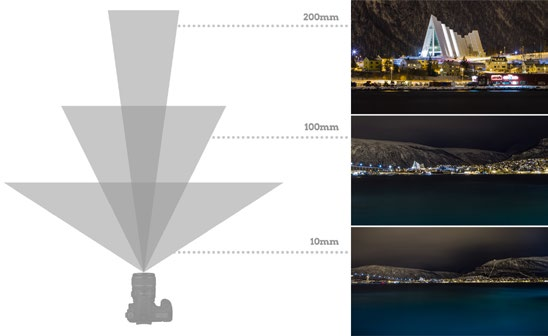
\includegraphics[width=0.7\linewidth]{figuras/revisaobiblio/claudia-distanciafocal}
	\label{fig:focaldistance}
	\fonte{\cite{man:claudia7licoes}.}
\end{figure}

Em um contexto de astrofotografia, lentes mais abertas são úteis para capturar a Via-Láctea (Figura \ref{fig:vialactea4mmSony}). Para fotografias de constelações, nebulosas e planetas distantes da Terra, é necessário uma lente mais fechada, que possibilite o enquadramento com o zoom necessário, conforme o tamanho do astro a ser fotografado. (Figura \ref{fig:jupiterSony})

\begin{figure}[!htb]
	\centering
	\caption{Fotografia da Via Láctea com lente \textit{zoom} em configuração de 4mm}
	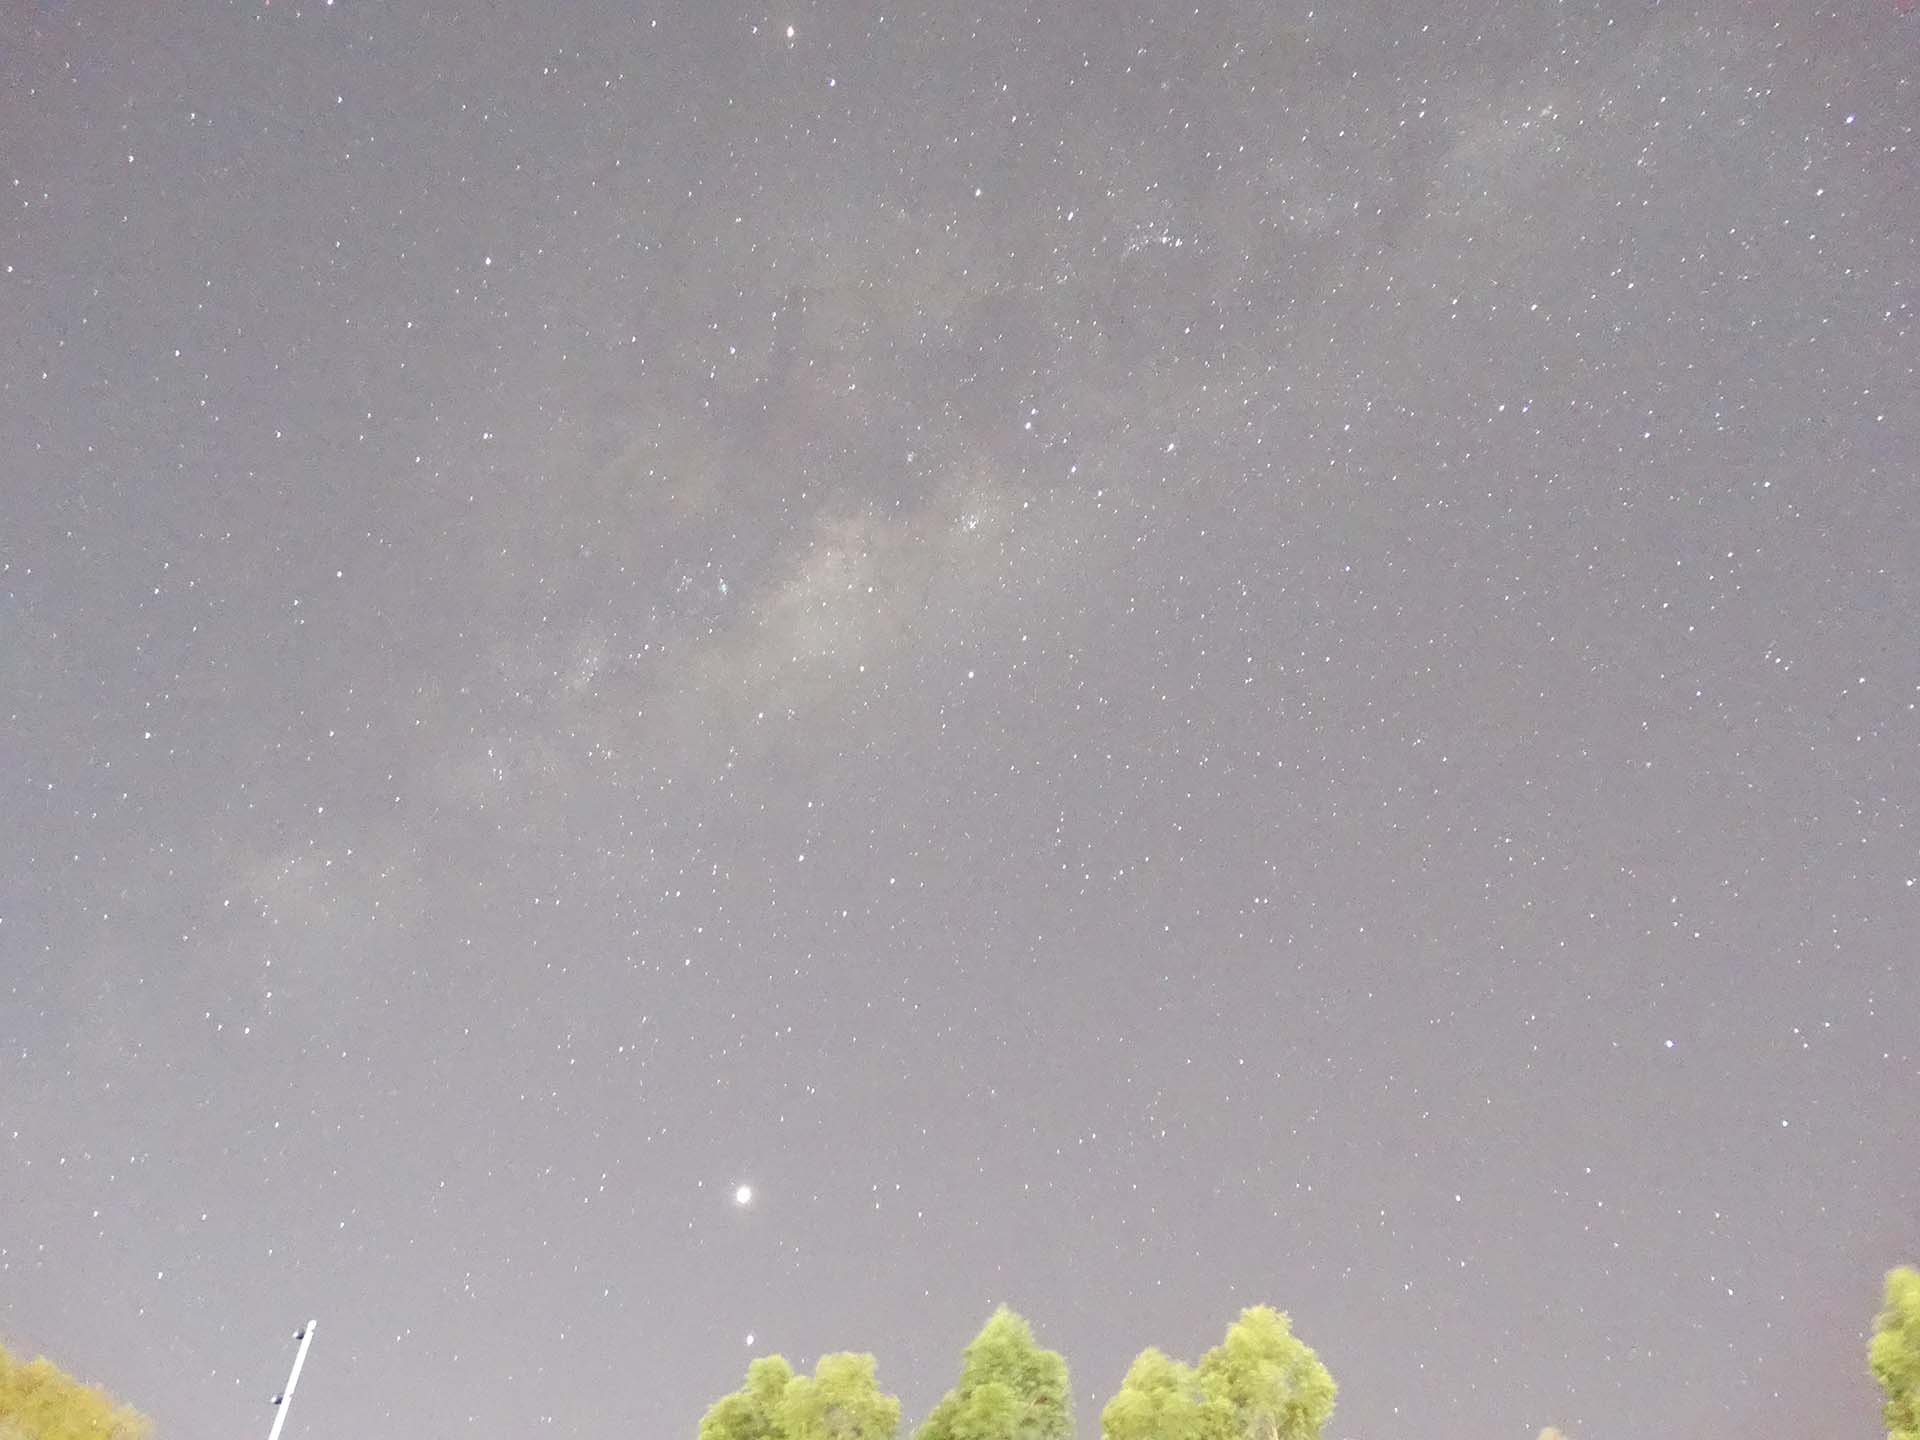
\includegraphics[width=0.7\linewidth]{figuras/revisaobiblio/vialactea4mm}
	\label{fig:vialactea4mmSony}
	\fonte{Autor.}
\end{figure}

\begin{figure}[!htb]
	\centering
	\caption{Fotografia de Júpiter e as Luas de Galileu com lente \textit{zoom} em configuração de 205mm}
	\includegraphics[width=0.2\linewidth]{figuras/revisaobiblio/jupiter205mm_Luas}
	\label{fig:jupiterSony}
	\fonte{Autor.}
\end{figure}

\subsection{Exposição}

A exposição de uma imagem se refere à quantidade de luz captada pelo sensor da câmera. Uma imagem muito clara é considerada superexposta, um caso onde o sensor recebeu muita luz. Ao contrário, uma imagem subexposta é uma fotografia escura que recebeu pouca luz. Existem 3 parâmetros configuráveis em uma câmera profissional que são determinantes para a exposição e também para a qualidade da foto final \cite{site:eduardoemonica}. De forma geral, conseguir a exposição ideal é o principal desafio da astrofotografia de céu profundo \cite{livro:astropratica}.


\subsubsection{Tempo de Exposição}

Para captar uma imagem, a câmera possui um dispositivo que permite a passagem de luz em direção ao sensor interno que capta a imagem. Uma fotografia de longa exposição significa que a câmera permaneceu captando luz por um longo intervalo de tempo \cite{book:bbcsky}. Porém, não é possível abusar de longas exposições em alguns casos, pois a imagem pode sair "borrada" (Figura \ref{fig:velocidade}). uma pessoa correndo precisa ser fotografada em uma fração de segundo e uma paisagem, ao contrário, pode ser capturada durante mais de um segundo se a câmera estiver imóvel em um tripé.  

\begin{figure}[!htb]
	\centering
	\caption{Impacto do tempo de exposição de captura para objetos em movimento}
	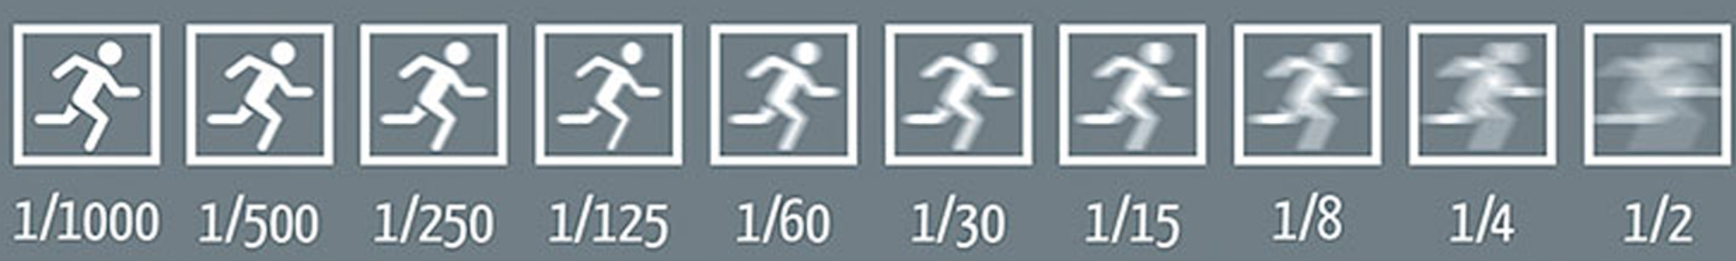
\includegraphics[width=0.9\linewidth]{figuras/revisaobiblio/velocidade}
	\label{fig:velocidade}
	\fonte{Adaptado de \cite{site:eduardoemonica}.}
\end{figure}

\subsubsection{Abertura}

Esse é o diâmetro do diafragme da lente, que permite a passagem de luz para o sensor (Figura \ref{fig:abertura}). Isso determina um valor "f/número". Um baixo "f/número" como f/1.8, indica um alto valor de abertura e significa dizer que a câmera irá receber mais luz \cite{book:bbcsky}. A abertura também impacta na profundidade de campo (Figura \ref{fig:profundidade}), o que significa que um valor baixo também apresenta o ônus da dificuldade focalizar.


\begin{figure}[!htb]
	\centering
	\caption{Variações de abertura de uma lente}
	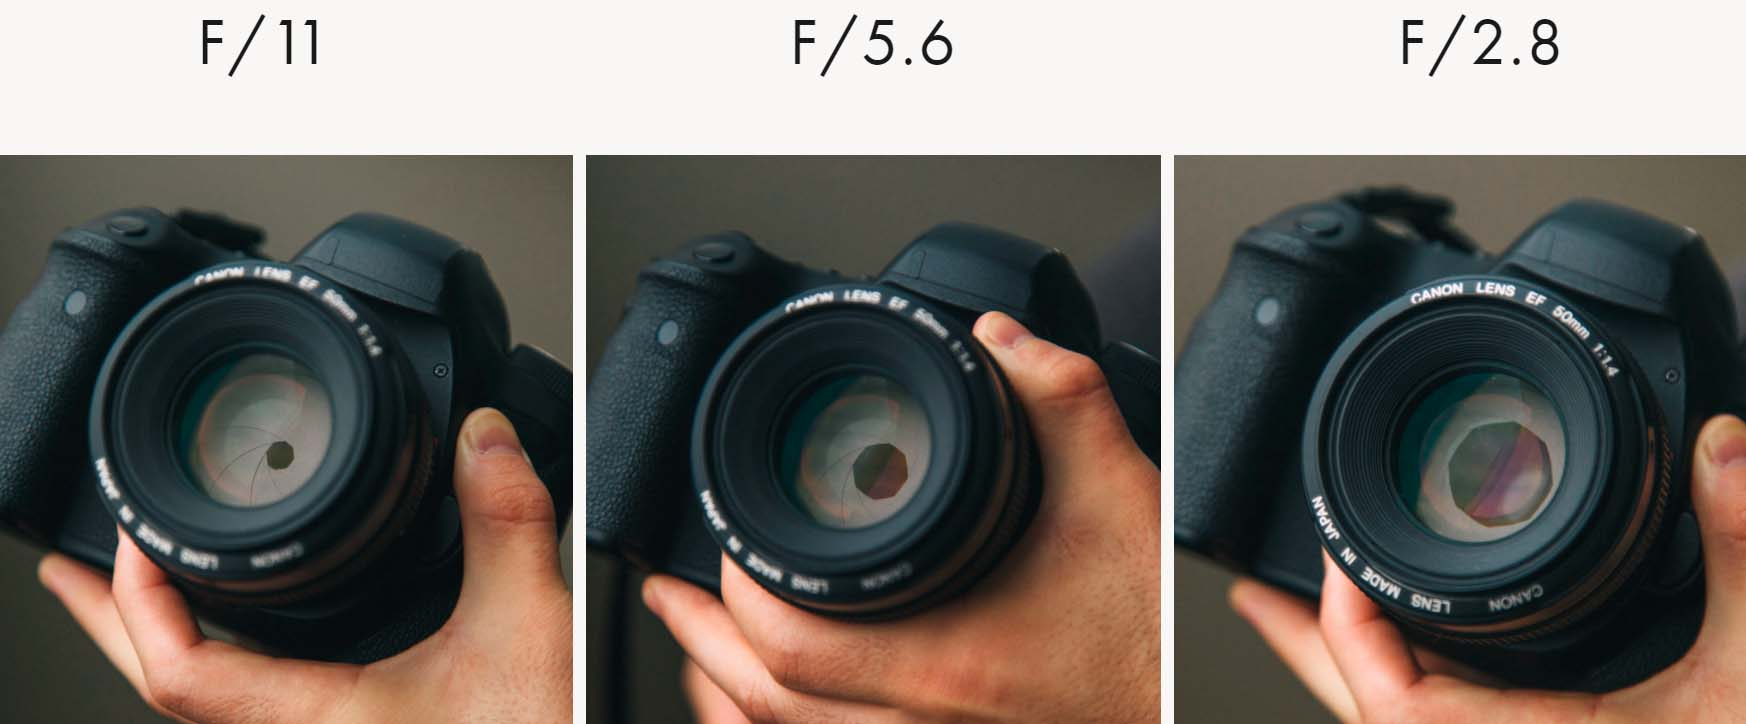
\includegraphics[width=0.7\linewidth]{figuras/revisaobiblio/abertura}
	\label{fig:abertura}
	\fonte{Adaptado de \cite{site:eduardoemonica}.}
\end{figure}

\begin{figure}[h]
	\centering
	\caption{Impacto da abertura na profundidade de campo}
	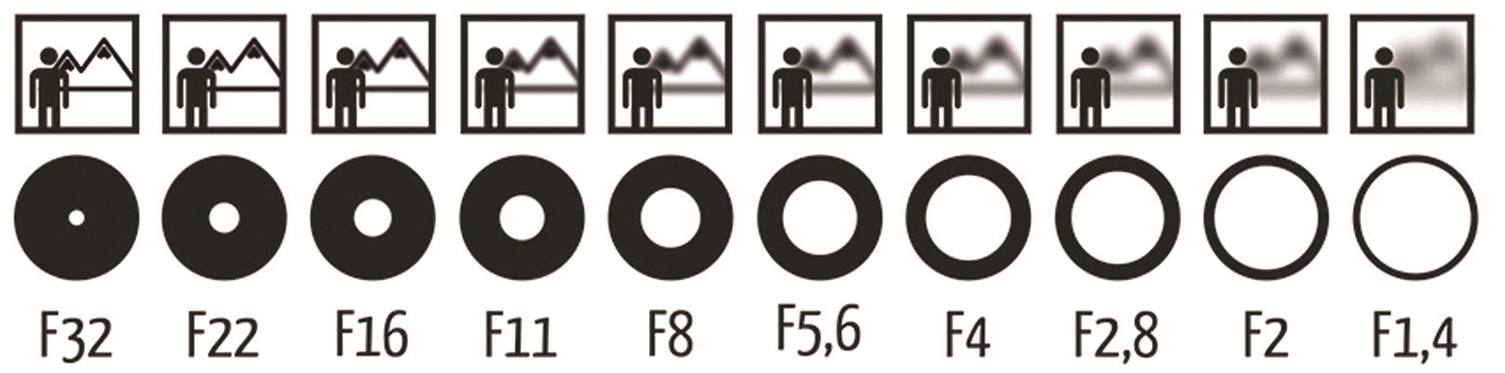
\includegraphics[width=0.9\linewidth]{figuras/revisaobiblio/profundidade}
	\label{fig:profundidade}
	\fonte{Adaptado de \cite{site:eduardoemonica}.}
\end{figure}

\subsubsection{Sensibilidade (ISO)}

O ISO é um padrão internacional para a sensibilidade do sensor das câmeras. Essa sensibilidade também é configurável no sistema da câmera no momento da fotografia. Um valor baixo de ISO significa que o sensor precisa de mais tempo de exposição para captar mais luz, ao mesmo tempo, que reduz o ruído na imagem. (Figura \ref{fig:iso})
Um valor de ISO alto implica que a imagem final terá muito ruído, mas possibilita que ela seja registrada com um baixo tempo de exposição \cite{book:bbcsky}. O ruído agregado pelo ISO também acaba prejudicando a fotografia, reduzindo o contraste e a saturação das imagens, o que também pode levar a posterização, que é o comprometimento total da fotografia, pois a foto perde resolução e criam-se falhas nos \textit{pixels} da imagem.


\begin{figure}[!htb]
	\centering
	\caption{Variações do ISO e o ruído agregado}
	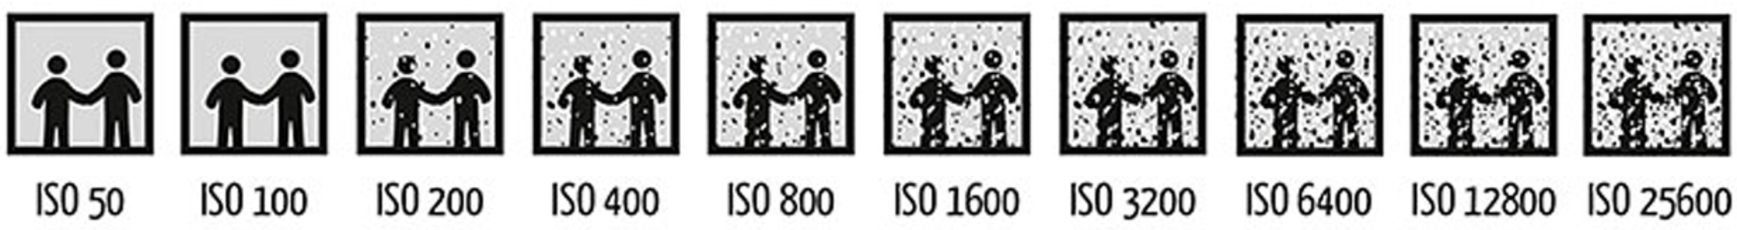
\includegraphics[width=0.9\linewidth]{figuras/revisaobiblio/ISO}
	\label{fig:iso}
	\fonte{Adaptado de \cite{site:eduardoemonica}.}
\end{figure}

\subsection{Formatos de Arquivos}

As câmeras profissionais possibilitam salvar as imagens em diferentes formatos de arquivos, que inclui formato RAW, JPG ou ambos. Os arquivos JPG são uma versão reduzida dos formatos RAW, onde se aplica um algoritmo de compressão de imagens que acaba gerando perca de informações. Desse modo, arquivos RAW possuem a informação completa do sensor, sem nenhum tipo de compactação e acabam sendo muito grandes, mas permitem uma pós-produção mais precisa que acaba resultando em uma imagem com mais qualidade e detalhes \cite{book:bbcsky}.

\subsection{Rastro de Estrelas}

O movimento de rotação da terra gera um movimento aparente no céu. Ao realizar uma fotografia de longa exposição, esse movimento será visível criando o efeito de rastro de estrelas ou \textit{star trail}. (Figura \ref{fig:startrail_example})

\begin{figure}[!htb]
	\centering
	\caption{Fotografia com a captura de um \textit{star trail}}
	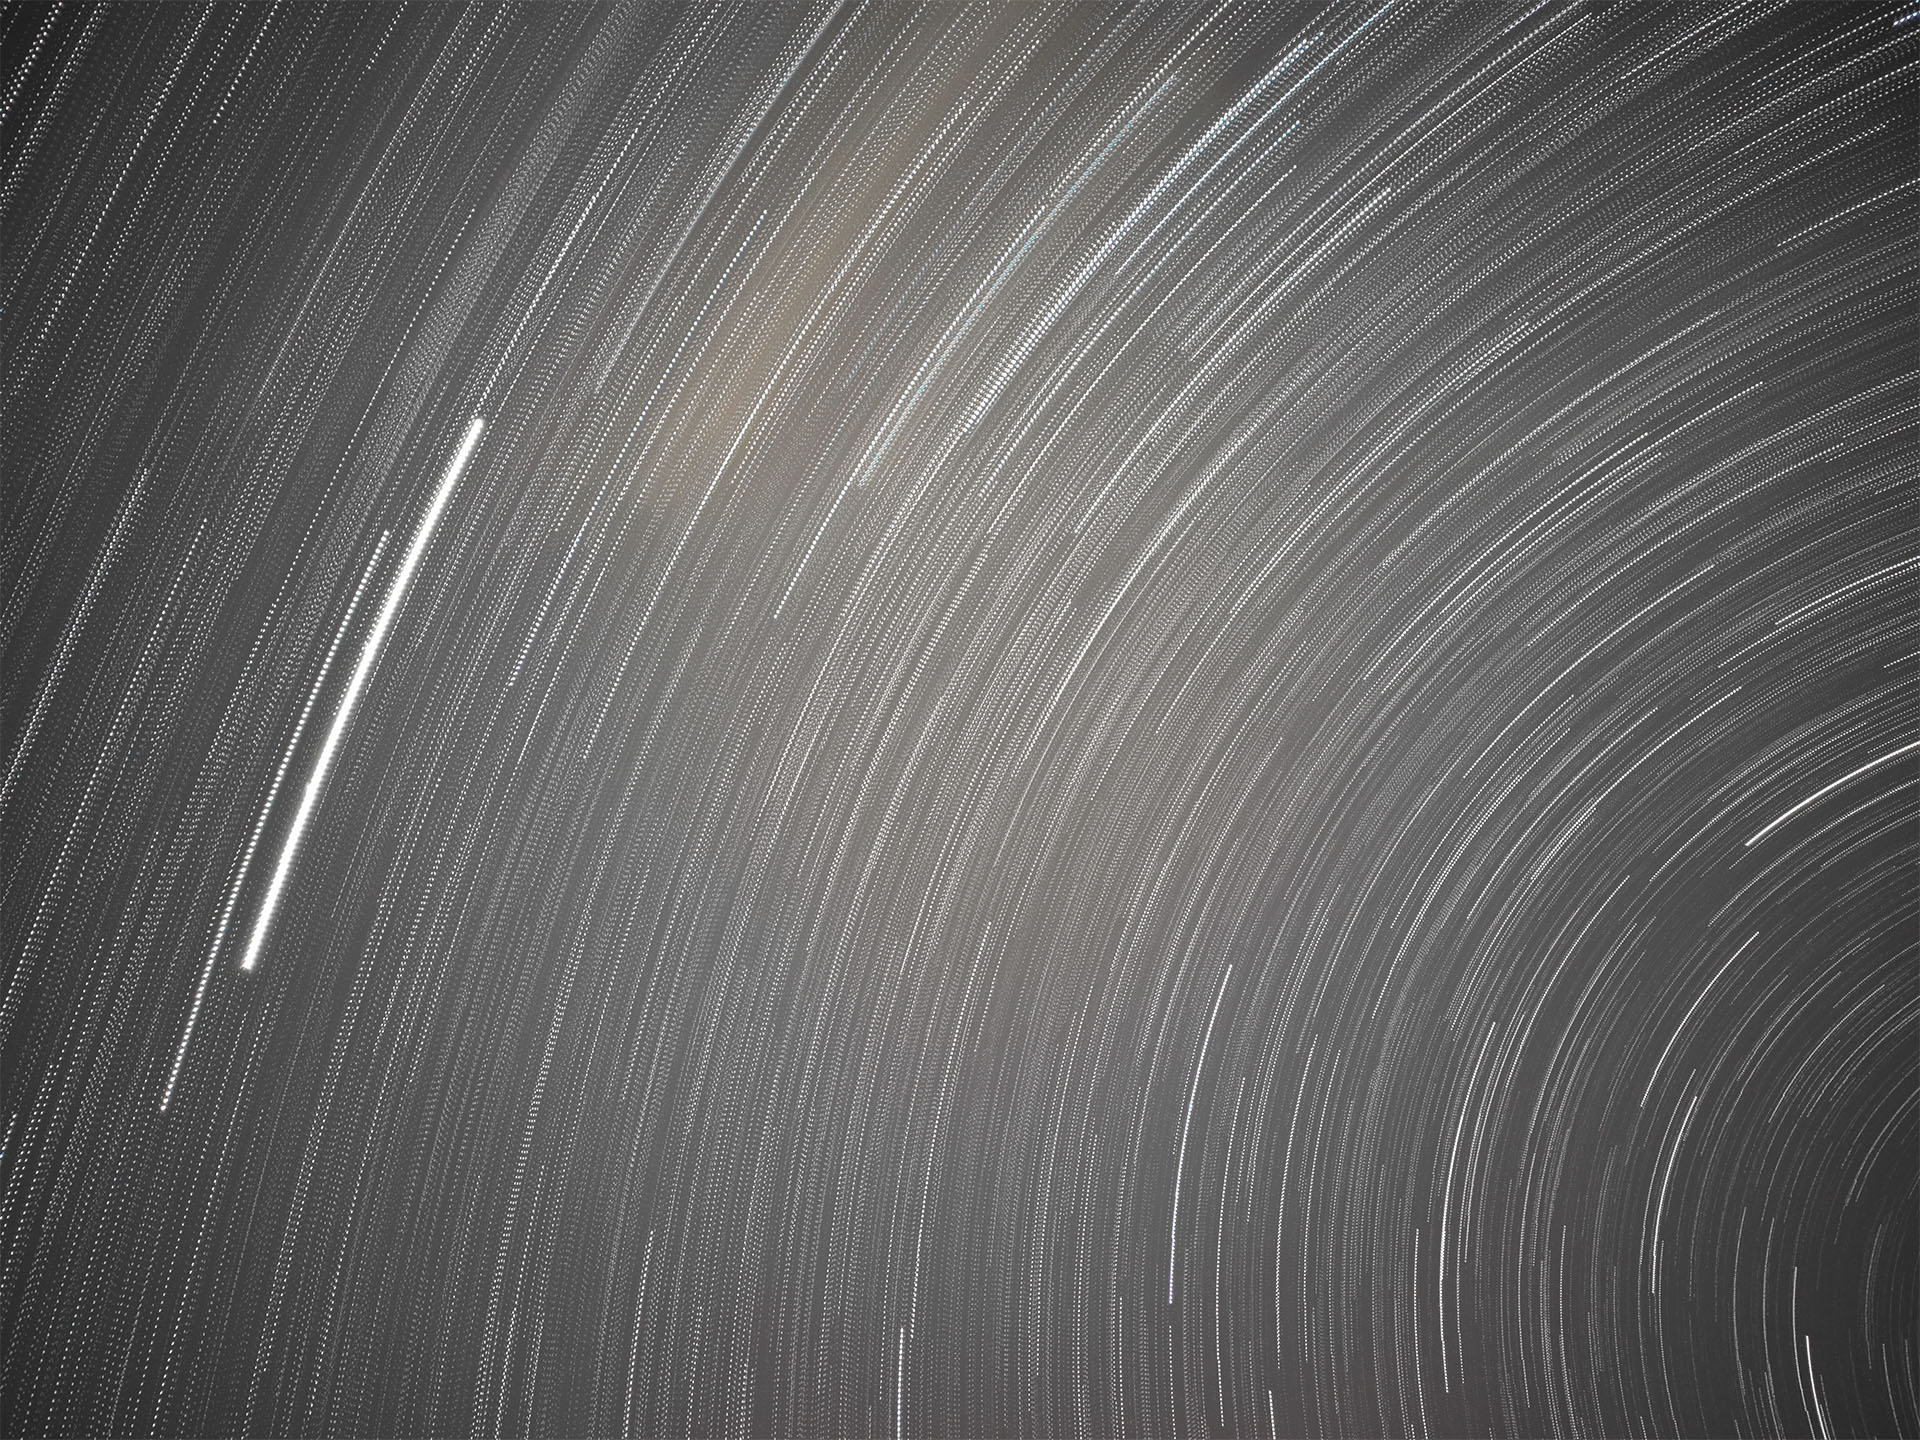
\includegraphics[width=0.7\linewidth]{figuras/revisaobiblio/startrail_example}
	\label{fig:startrail_example}
	\fonte{Autor.}
\end{figure}

\subsubsection{Tempo de Exposição Máximo}
\label{sec:TempoMax}

Existe um limite de tempo máximo para que uma câmera fixa permaneça capturando luz sem que ocorra o fenômeno de \textit{star trail}. Esse tempo máximo depende de vários fatores, mas os dois principais são a distância focal da lente e a posição da estrela.

A distância focal é importante pois uma lente com um longo comprimento amplia a imagem, da mesma forma que amplia o rastro das estrelas. Do contrário, lentes com ângulo mais aberto, de menor comprimento focal, fazem tudo parecer pequeno, incluindo o movimento das estrelas, e isso permite um tempo de exposição maior \cite{book:astrophotographyAmateur}.

A distância de um astro até a linha do equador celestial é chamada de declinação estrelar, sendo medida em graus. Quanto menor for essa distância, mais rápido a estrela aparenta se movimentar no céu. Seja a declinação simbolizada por $\sigma$, e a distância focal nomeado $F$, em milímetros , uma equação capaz de aproximar o limite do tempo de exposição é dada em (\ref{eq:timeexp}) \cite{book:astrophotographyAmateur}. Existem ainda outras metodologias que buscam aproximar o tempo máximo de exposição. 

\begin{equation}
	t_{max} = \dfrac{343}{F\cos(\sigma)}~~[s]
	\label{eq:timeexp}
\end{equation}



\paragraph{Regra dos 500}

A regra dos 500 é uma fórmula que se baseia apenas distância focal, e o cálculo do tempo máximo é dado pela equação \ref{eq:timeexp500}. É uma regra muito simples, mas que permite uma aproximação razoável sobre o tempo máximo de exposição. Existem variantes dessa regra que alteram a constante no numerador, como a regra dos 300 ou a regra dos 400 \cite{site:500xNPF}.

\begin{equation}
	t_{max} = \dfrac{500}{F}~~[s]
	\label{eq:timeexp500}
\end{equation}

\paragraph{Regra NPF}

A regra NPF é uma evolução da equação (\ref{eq:timeexp}), que considera múltiplos fatores para recalcular a constante do numerador
\cite{site:500xNPF}. O tempo de exposição máximo é calculado pela equação \ref{eq:npf} com base na abertura da lente ($ N $), na distância focal ($ F $), no tamanho em micrômetros do sensor da câmera ($ p $), na declinação da estrela para onde a câmera será apontada ($\sigma$), e um fator de multiplicação ($ k $). O fator $ k $ é mantido em 1, porém pode ser aumentado até 3 para obter imagens mais nítidas e contrastantes \cite{site:500xNPF}. 

\begin{equation}
	t_{max} = k \cdot \dfrac{16,9 N  + 0,1 F + 13,7 p}{F\cos(\sigma)}~~[s]
	\label{eq:npf}
\end{equation}

\subsection{Empilhamento de Fotos}

O fenômeno de \textit{star trail} gera a necessidade do uso de ferramentas para compensar o movimento da Terra e permitir uma fotografia de longa exposição sem que se crie rastro. Essa compensação pode ser feita por \textit{software}, realizando-se o empilhamento de fotos de curta exposição \cite{livro:astropratica}.

O empilhamento consiste na junção de múltiplas imagens capturadas com a câmera montada em um tripé ou em uma montagem motorizada, que possibilita o somatório da luz capturada com essas fotos. Esse método de processamento é relevante para qualquer astrofotografia e possibilita a redução de ruído usando imagens de calibração \cite{book:bbcsky}. Existem inúmeros programas capazes de realizar esse processo como \textit{Deep Sky Stacker}, \textit{Sequator}, entre outros.

A combinação das imagens no pós-processamento não gera uma imagem mais luminosa ou colorida, o objetivo da combinação é o aumento da Relação Sinal Ruído (SNR). A única forma de gerar uma imagem final com mais luz e cores é realizando uma sequência de fotografias com maior tempo de exposição \cite{man:deepskystackerBetterImages}. As figuras \ref{noCalibration} e \ref{withCalibration} comparam o resultado de uma imagem que passou pelo processo de empilhamento. 

\begin{figure}[!htb]
	\centering
	\caption{Efeito da combinação de imagens. (a) Imagem Original e (b) Empilhamento de 32 imagens}
	\captionsetup[subfigure]{justification=centering}
	\begin{subfigure}[b]{0.49\textwidth}
		\centering
		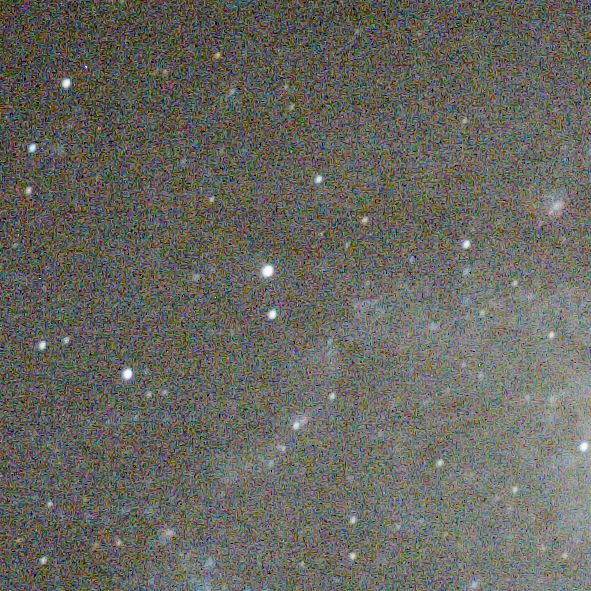
\includegraphics[width=\textwidth]{figuras/revisaobiblio/Stack_1}
		\caption{}
		\label{noCalibration}
	\end{subfigure}
 	\hfill
 	\begin{subfigure}[b]{0.49\textwidth}
 		\centering
	 	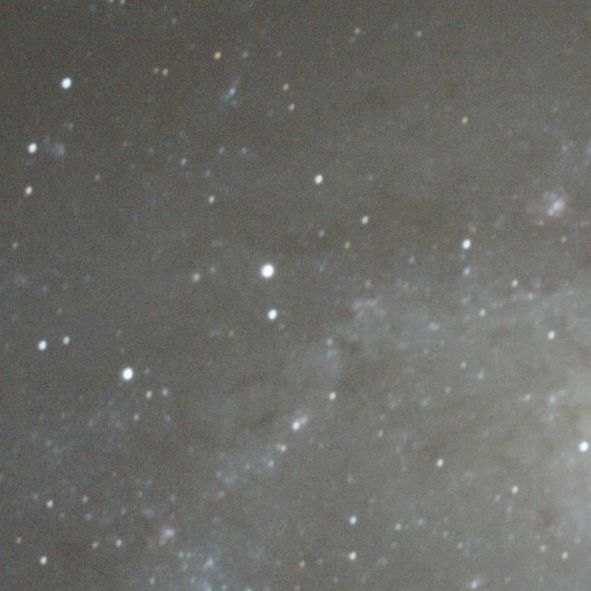
\includegraphics[width=\textwidth]{figuras/revisaobiblio/Stack_32}
	 	\caption{}
	 	\label{withCalibration}
	 \end{subfigure}

	\fonte{\cite{man:deepskystackerBetterImages}.}
\end{figure}


\subsubsection{Imagens de Calibração}

As fotografias registradas sobre um alvo celeste são chamadas de \textit{Light Frames} e estas podem ser empilhadas como escrito anteriormente. No entanto, é possível realizar um processo de calibração do empilhamento, fornecendo imagens de calibração \cite{man:deepskystackerfaq}.
O processo é feito combinando fotos chamadas de \textit{Dark Frames},\textit{ Bias Frames}, \textit{Flat Frames} e \textit{Dark Flat Frames} (não muito utilizado). Essas imagens são extras e precisam ser fotografadas com a câmera em condições específicas e posteriormente adicionadas ao \textit{software} durante o processo de empilhamento 
\cite{man:deepskystackerBetterImages}. O resultado entregue pelo \textit{software} será uma imagem final calibrada, como demonstra o diagrama da Figura \ref{fig:calibrationDeepSkyStacker}.

% todo refazer imagem

\begin{figure}[!htb]
	\centering
	\caption{Diagrama do processo de calibração do empilhamento sem o uso de \textit{Dark Flat Frames}}
	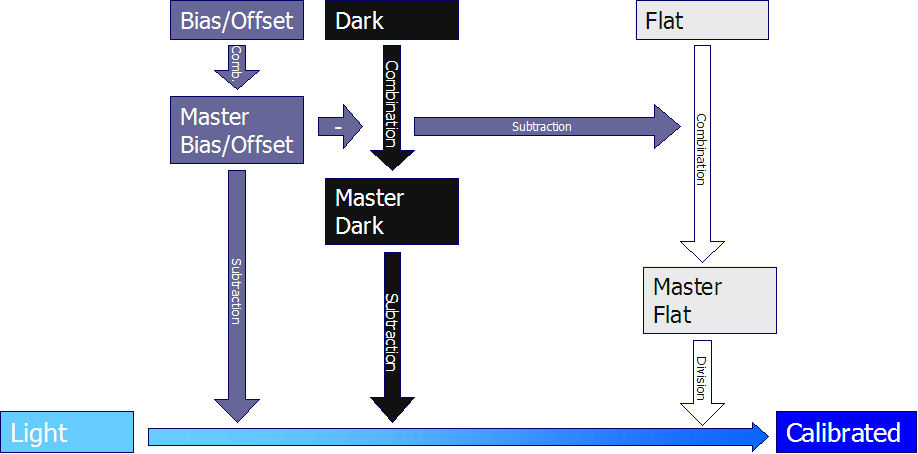
\includegraphics[width=0.9\linewidth]{figuras/revisaobiblio/Calibration_Alternate1}
	\label{fig:calibrationDeepSkyStacker}
	\fonte{Adaptado de \cite{man:deepskystackerBetterImages}.}
\end{figure}


\paragraph{\textit{Dark Frames}}

Os \textit{Dark Frames} são fotografias que indicam ao software a localização do sinal de ruído das fotografias. São necessárias de 10 a 20 fotos com a lente tampada para criar a calibração, as quais devem necessariamente ser fotografadas com ISO, tempo de exposição e condições ambientais iguais aos \textit{light frames}.\cite{man:deepskystackerfaq}

\paragraph{\textit{Bias (Offset) Frames}}

Os \textit{Bias/Offset Frames} são usados para remover sinais de ruído na leitura do sensor da câmera. Essas fotografias devem ser capturadas no menor tempo de exposição possível, com lente tampada, na mesma configuração de ISO dos \textit{Light Frames}. São necessárias cerca de 10 a 20 fotos para que a calibração funcione adequadamente. A temperatura da câmera não é um fator relevante nesse caso \cite{man:deepskystackerfaq}.


\paragraph{\textit{Flat Frames}}
\textit{Flat Frames} são imagens de calibração capturadas com mesmo ISO e abertura dos \textit{light frames} colocando uma folha branca na frente da lente, incidindo luz na folha. Elas têm o objetivo de indicar a vinheta da lente(escurecimento nas bordas da imagem), além da distribuição não uniforme de luz provocada por pó ou riscos na lente. Novamente, são necessários de 10 a 20 imagens
\cite{man:deepskystackerfaq}.


\subsection{Métodos de Rastreamento}

Tendo em vista o limite do tempo de exposição e o movimento de rotação da Terra, discutidos na seção \ref{sec:TempoMax}, os \textit{softwares} de empilhamento possuem algoritmos que compensam a rotação das estrelas, rotacionando as imagens fotografadas no sentido oposto, e realizando o empilhamento dessas imagens após esse ajuste das fotos. Esse método compensa o ruído, mas como os tempos de exposições são curtos, torna-se mais difícil obter cor e contrastes nos objetos celestes. Isso só é possível capturar aumentando o tempo de exposição. 

Então, para realizar astrofotografias de longa exposição, é necessário o uso de um rastreador físico que movimenta a câmera no sentido de rotação aparente das estrelas, garantindo que não ocorrerá o efeito de \textit{star trail}. Existem dois métodos de rastreamento: Alt-Azimutal e Equatorial \cite{book:bbcsky}.

\subsubsection{Alt-Azimutal}

Uma montagem Alt-Azimutal funciona movendo uma câmera ou um telescópio por meio dos eixos vertical e horizontal, alterando o azimute e a altitude simultaneamente. Isso requer um sistema com dois motores para realizar o rastreamento, o que torna essa montagem mais cara e complexa. Além disso, para astrofotografias, essa montagem acaba não sendo indicada pois ela não consegue compensar a rotação aparente dos astros, que também é gerado pelo movimento de rotação da terra (Figura \ref{fig:altazimuterotation}) \cite{book:bbcsky}. 

\begin{figure}[!htb]
	\centering
	\caption{O enquadramento não rotaciona com o astro na montagem Alt-Azimutal}
	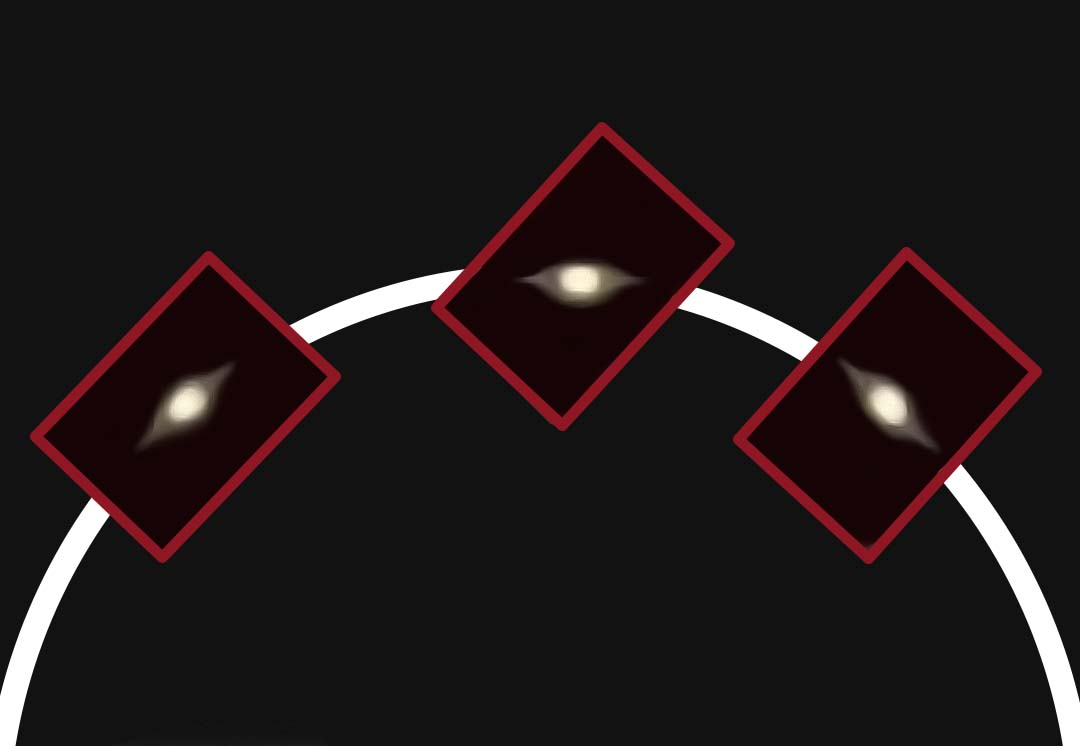
\includegraphics[width=0.45\linewidth]{figuras/revisaobiblio/altazimuterotation}
	\label{fig:altazimuterotation}
	\fonte{Adaptado de \cite{book:bbcsky}.}
\end{figure}


\subsubsection{Equatorial}

Ao contrário do modelo de montagem comentado na seção anterior, uma montagem equatorial consegue compensar a rotação aparente dos astros (Figura \ref{fig:equatorialrotation}) e, por esse motivo, é a melhor opção de mecanismo para realizar astrofotografias. Isso ocorre pois essa construção realiza o movimento da câmera de forma circular, na mesma velocidade de rotação aparente da Terra, após alinhar o eixo de altitude junto com o meridiano polar (eixo norte-sul) \cite{book:bbcsky}. Esse sistema requer somente um motor, porém, precisa também de um método acurado de alinhamento com o meridiano e isso será explorado na próxima seção. 

\begin{figure}[!htb]
	\centering
	\caption{O enquadramento se mantêm constante na montagem equatorial}
	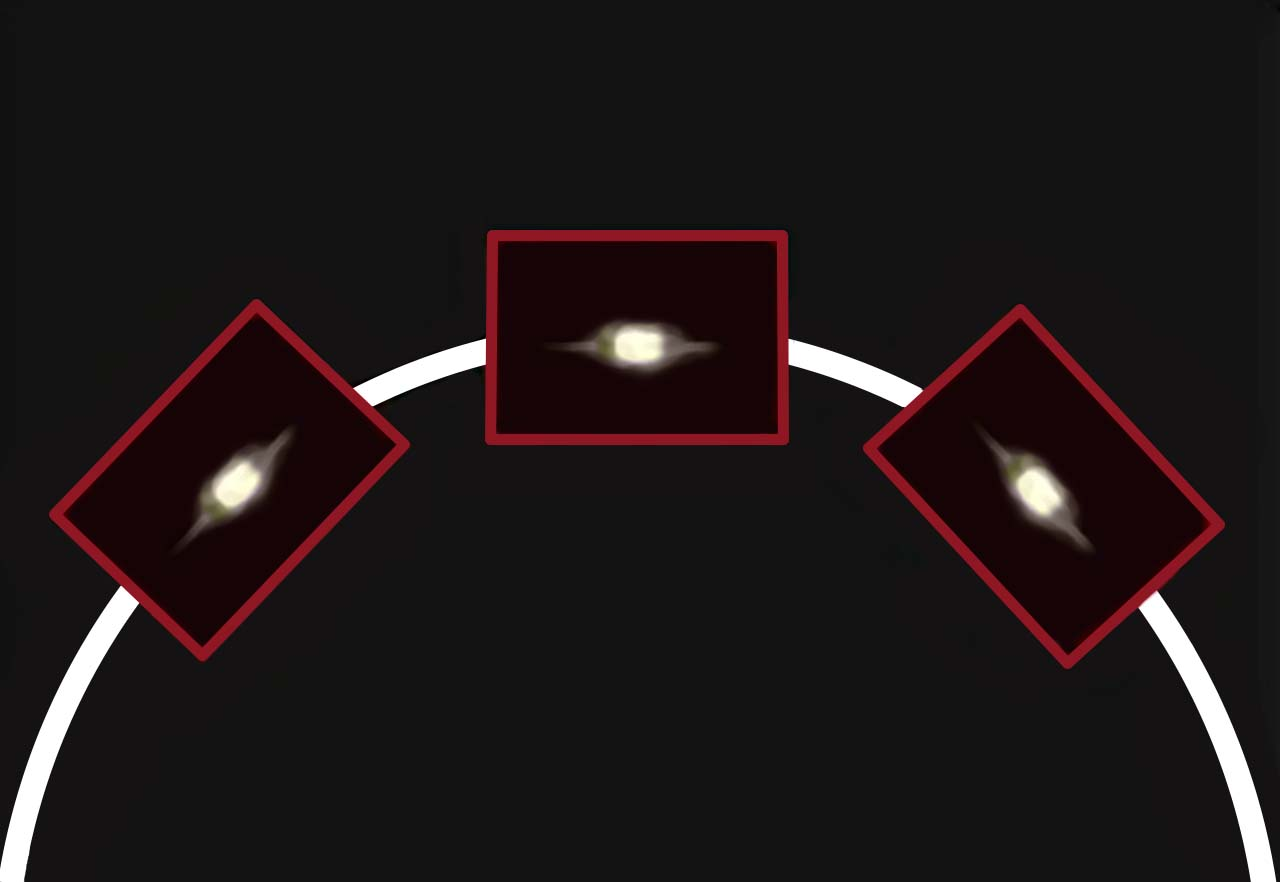
\includegraphics[width=0.45\linewidth]{figuras/revisaobiblio/equatorialrotation}
	\label{fig:equatorialrotation}
	\fonte{Adaptado de \cite{book:bbcsky}.}
\end{figure}

\section{Plataformas Equatoriais}

Plataformas Equatoriais são mecanismos que se baseiam em uma montagem equatorial para realizar o rastreamento das estrelas no céu. Existem modelos para telescópios e outros específicos para astrofotografia, sendo este último o foco deste trabalho. Essa montagem requer o alinhamento do eixo de rotação da plataforma com o eixo de rotação celeste que, para uma pessoa localizada no hemisfério norte, será o polo norte polar, e para alguém no hemisfério sul, será o polo sul polar (Figura \ref{fig:celestialchart}). 

\begin{figure}[!htb]
	\centering
	\caption{A posição do polo norte/sul celestial, no céu, depende da posição geográfica (latitude) da pessoa/equipamento de observação e é alinhado com o eixo de rotação da terra.}
	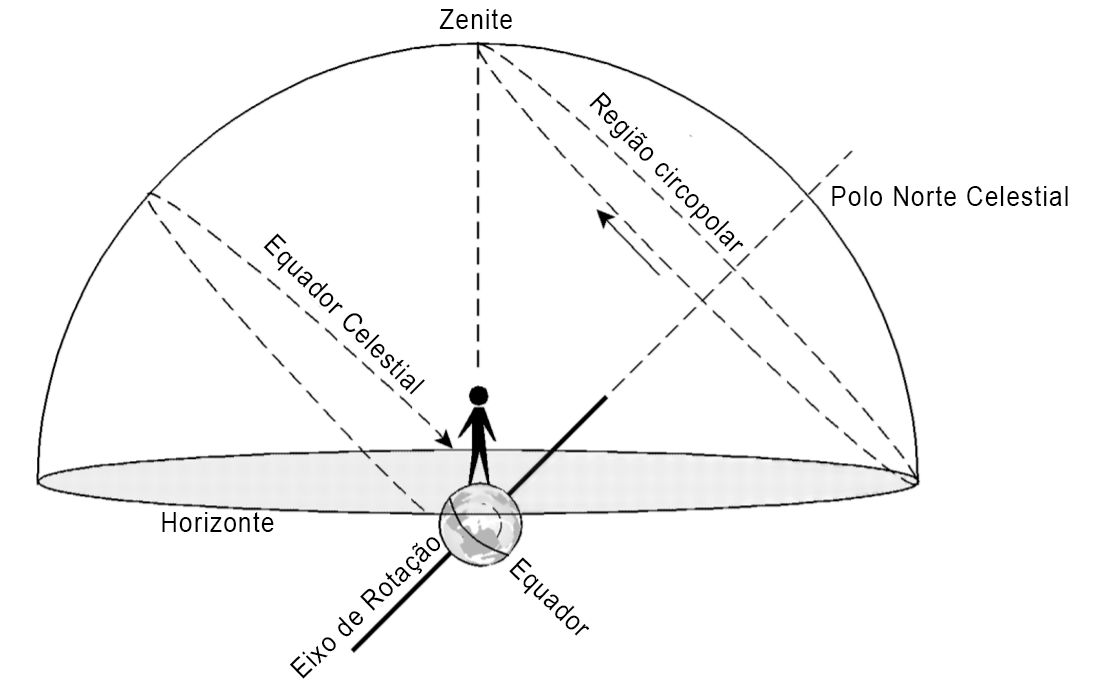
\includegraphics[width=0.8\linewidth]{figuras/revisaobiblio/celestialchart}
	\label{fig:celestialchart}
	\fonte{\cite{livro:starwatch:v1}.}
\end{figure}

Depois que o eixo da plataforma está alinhado com o polo celeste, ela começa a rotacionar no sentido e mesma taxa da rotação do planeta.

\subsection[Modelos de Montagem]{Modelos de Montagem \textit{Barn Door}}
\textit{Barn Door} é um modelo de montagem que se caracterizam por funcionar com duas bases acopladas, onde uma é fixada no tripé do fotógrafo, e a outra é móvel, fixando a câmera que será rotacionada para acompanhar o movimento aparente do céu (Figura \ref{fig:barndoorexample}). O funcionamento é igual a abertura de uma porta com dobradiças \cite{site:pentaxBarnDoor}. 

\begin{figure}[!htb]
	\centering
	\caption{Exemplo de Montagem \textit{Barn Door}}
	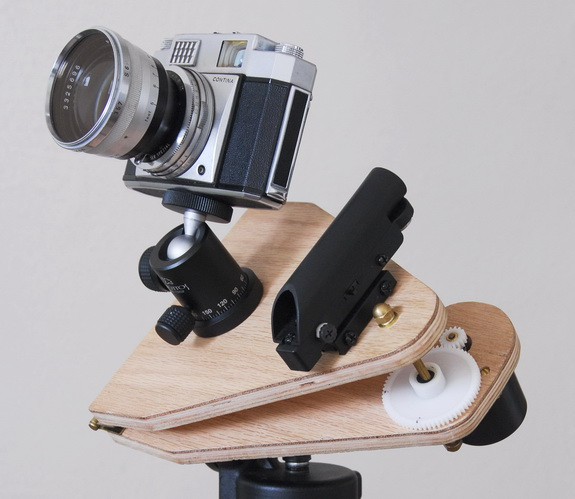
\includegraphics[width=0.5\linewidth]{figuras/revisaobiblio/barndoorexample}
	\label{fig:barndoorexample}
	\fonte{\cite{artigo:garySeronik}.}
\end{figure}


Esses modelos são tradicionalmente conhecidos pela comunidade de astrofotografia por serem de baixo custo, pois é possível automatizar o movimento da câmera sem a necessidade de um motor demasiadamente potente e caro. Além disso, comparando a modelos de montagem usado em sistemas comerciais, um sistema \textit{Barn Door} pode ser facilmente modificado ou reparado. Perdem para modelos comerciais no quesito transportabilidade e precisão \cite{site:pentaxBarnDoor}. A transportabilidade é a facilidade com que o equipamento pode ser transportado de um ponto ao outro, isso leva em conta o formato da estrutura, volume e peso.
 
Dentre os modelos de \textit{Barn Door}, os mais comuns são: montagem com braço simples; montagem com braço Duplo e montagem curva. A primeira (Figura \ref{fig:singleArm}) é composta por uma base fixa conectada a base da câmera que é movida por um eixo perpendicular à parte fixa. Esse sistema acaba tendo algumas limitações para manter uma variação constante no ângulo de rotação da câmera, que, apesar da elevação do eixo ser constante, o ângulo de rotação não é, o que acumulará erro de rastreamento. Isso gera erros de rastreamento que limitam o uso desse modelo para exposições com, no máximo, 15 minutos \cite{artigo:davidtrottinventions}. 

\begin{figure}[!htb]
	\centering
	\caption{\textit{Barn Door} com braço simples}
	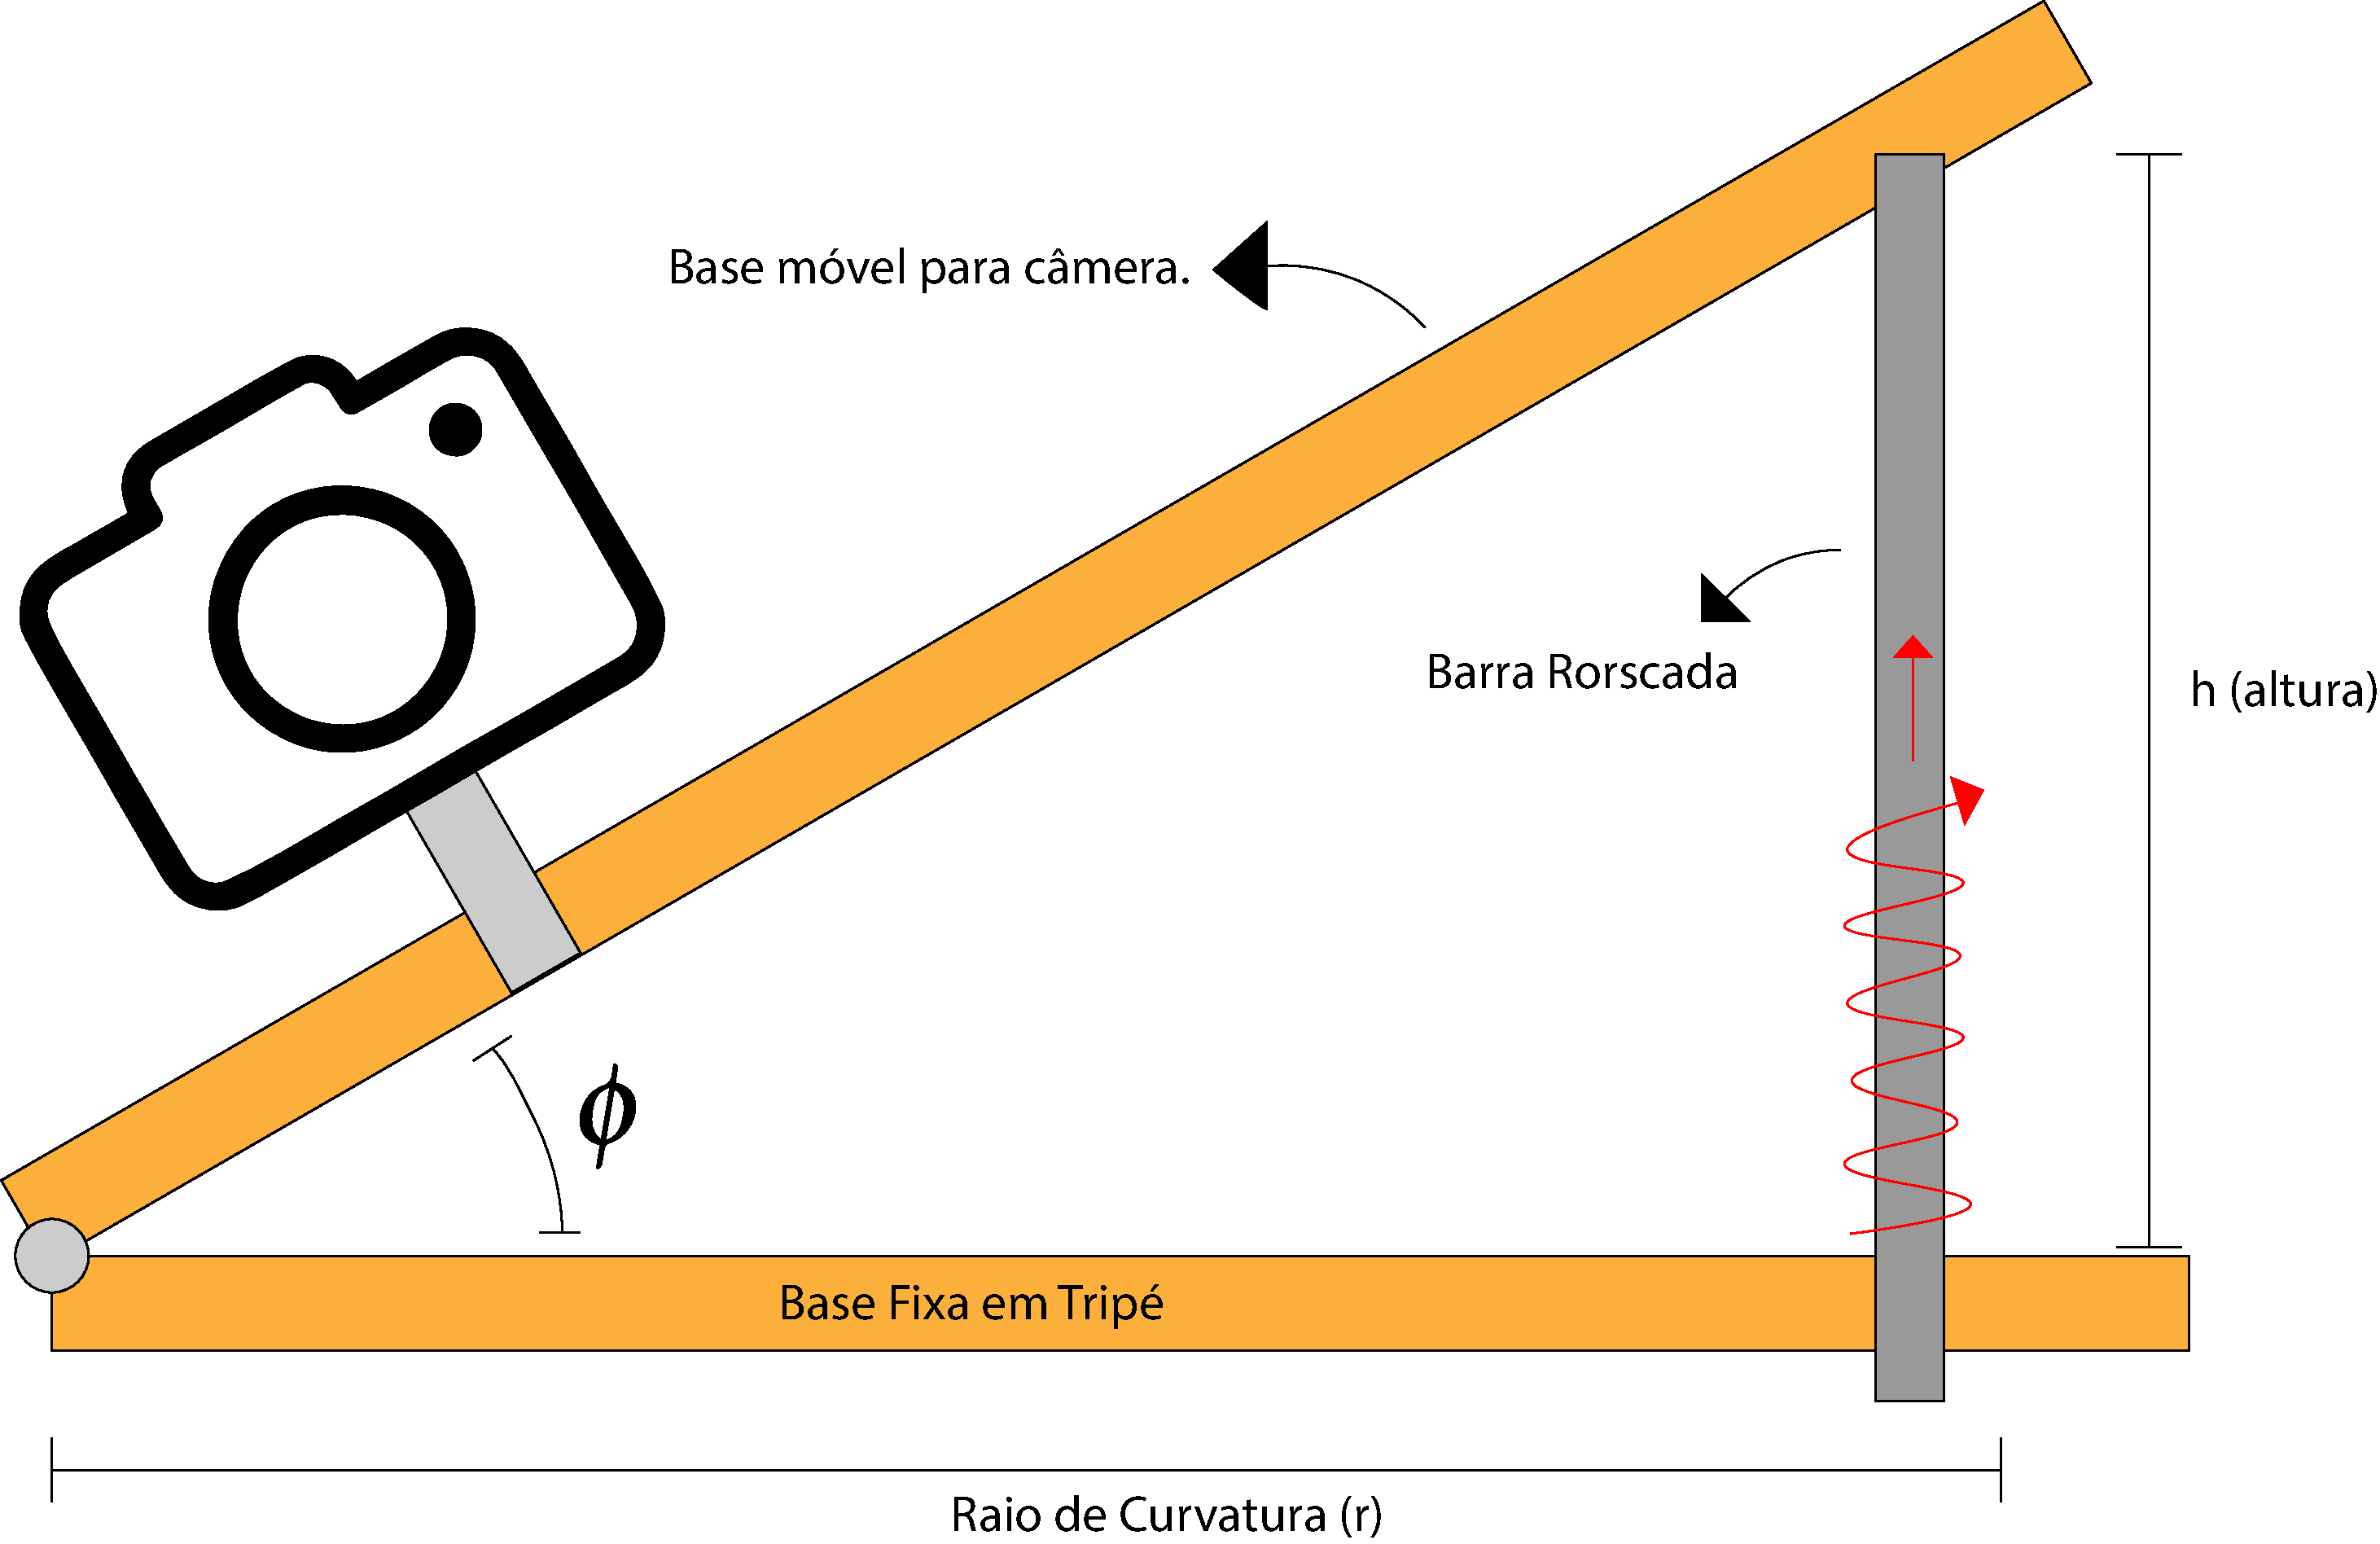
\includegraphics[width=0.6\linewidth]{figuras/revisaobiblio/bracosimples}
	\label{fig:singleArm}
	\fonte{Adaptado de \cite{artigo:davidtrottinventions}.}
\end{figure}

Trot (1989) desenvolveu um mecanismo de braço duplo (Figura \ref{fig:doublearm}) que consegue aumentar para até 1h o tempo máximo de exposição, em comparação com o modelo anterior. Contudo, tem como desvantagem a complexidade do sistema, que exige várias peças o que pode se tornar demasiadamente complexo para montagem e configuração.

\begin{figure}[!htb]
	\centering
	\caption{Diagrama de montagem do mecanismo de Braço Duplo}
	\includegraphics[width=0.6\linewidth]{figuras/revisaobiblio/heavy-duty-double-arm-barndoor-building-plans-3_edited}
	\label{fig:doublearm}
	\fonte{Adaptado de \cite{artigo:davidtrottinventions}.}
\end{figure}

Por fim, a montagem curva é composta por uma barra roscada curva, que não possui o problema de compensação de velocidade, pois ela acompanha a curvatura do movimento da plataforma. A dificuldade dessa montagem provém da curvatura do eixo de rotação, que pode trazer questões relacionadas à estabilidade devido à necessidade de folga nas bases (Figura \ref{fig:montagemCurva}). Outro detalhe é que a barra não pode ser rotacionada. A movimentação deve ser feita através de uma rosca que é rotacionada na base, e realiza o deslocamento da barra rosqueada para cima ou para baixo \cite{site:pentaxBarnDoor}.  

 
 \begin{figure}[!htb]
 	\centering
 	\caption[Modelo de Montagem Curva]{Modelo de Montagem Curva e o problema da folga no mecanismo}
 	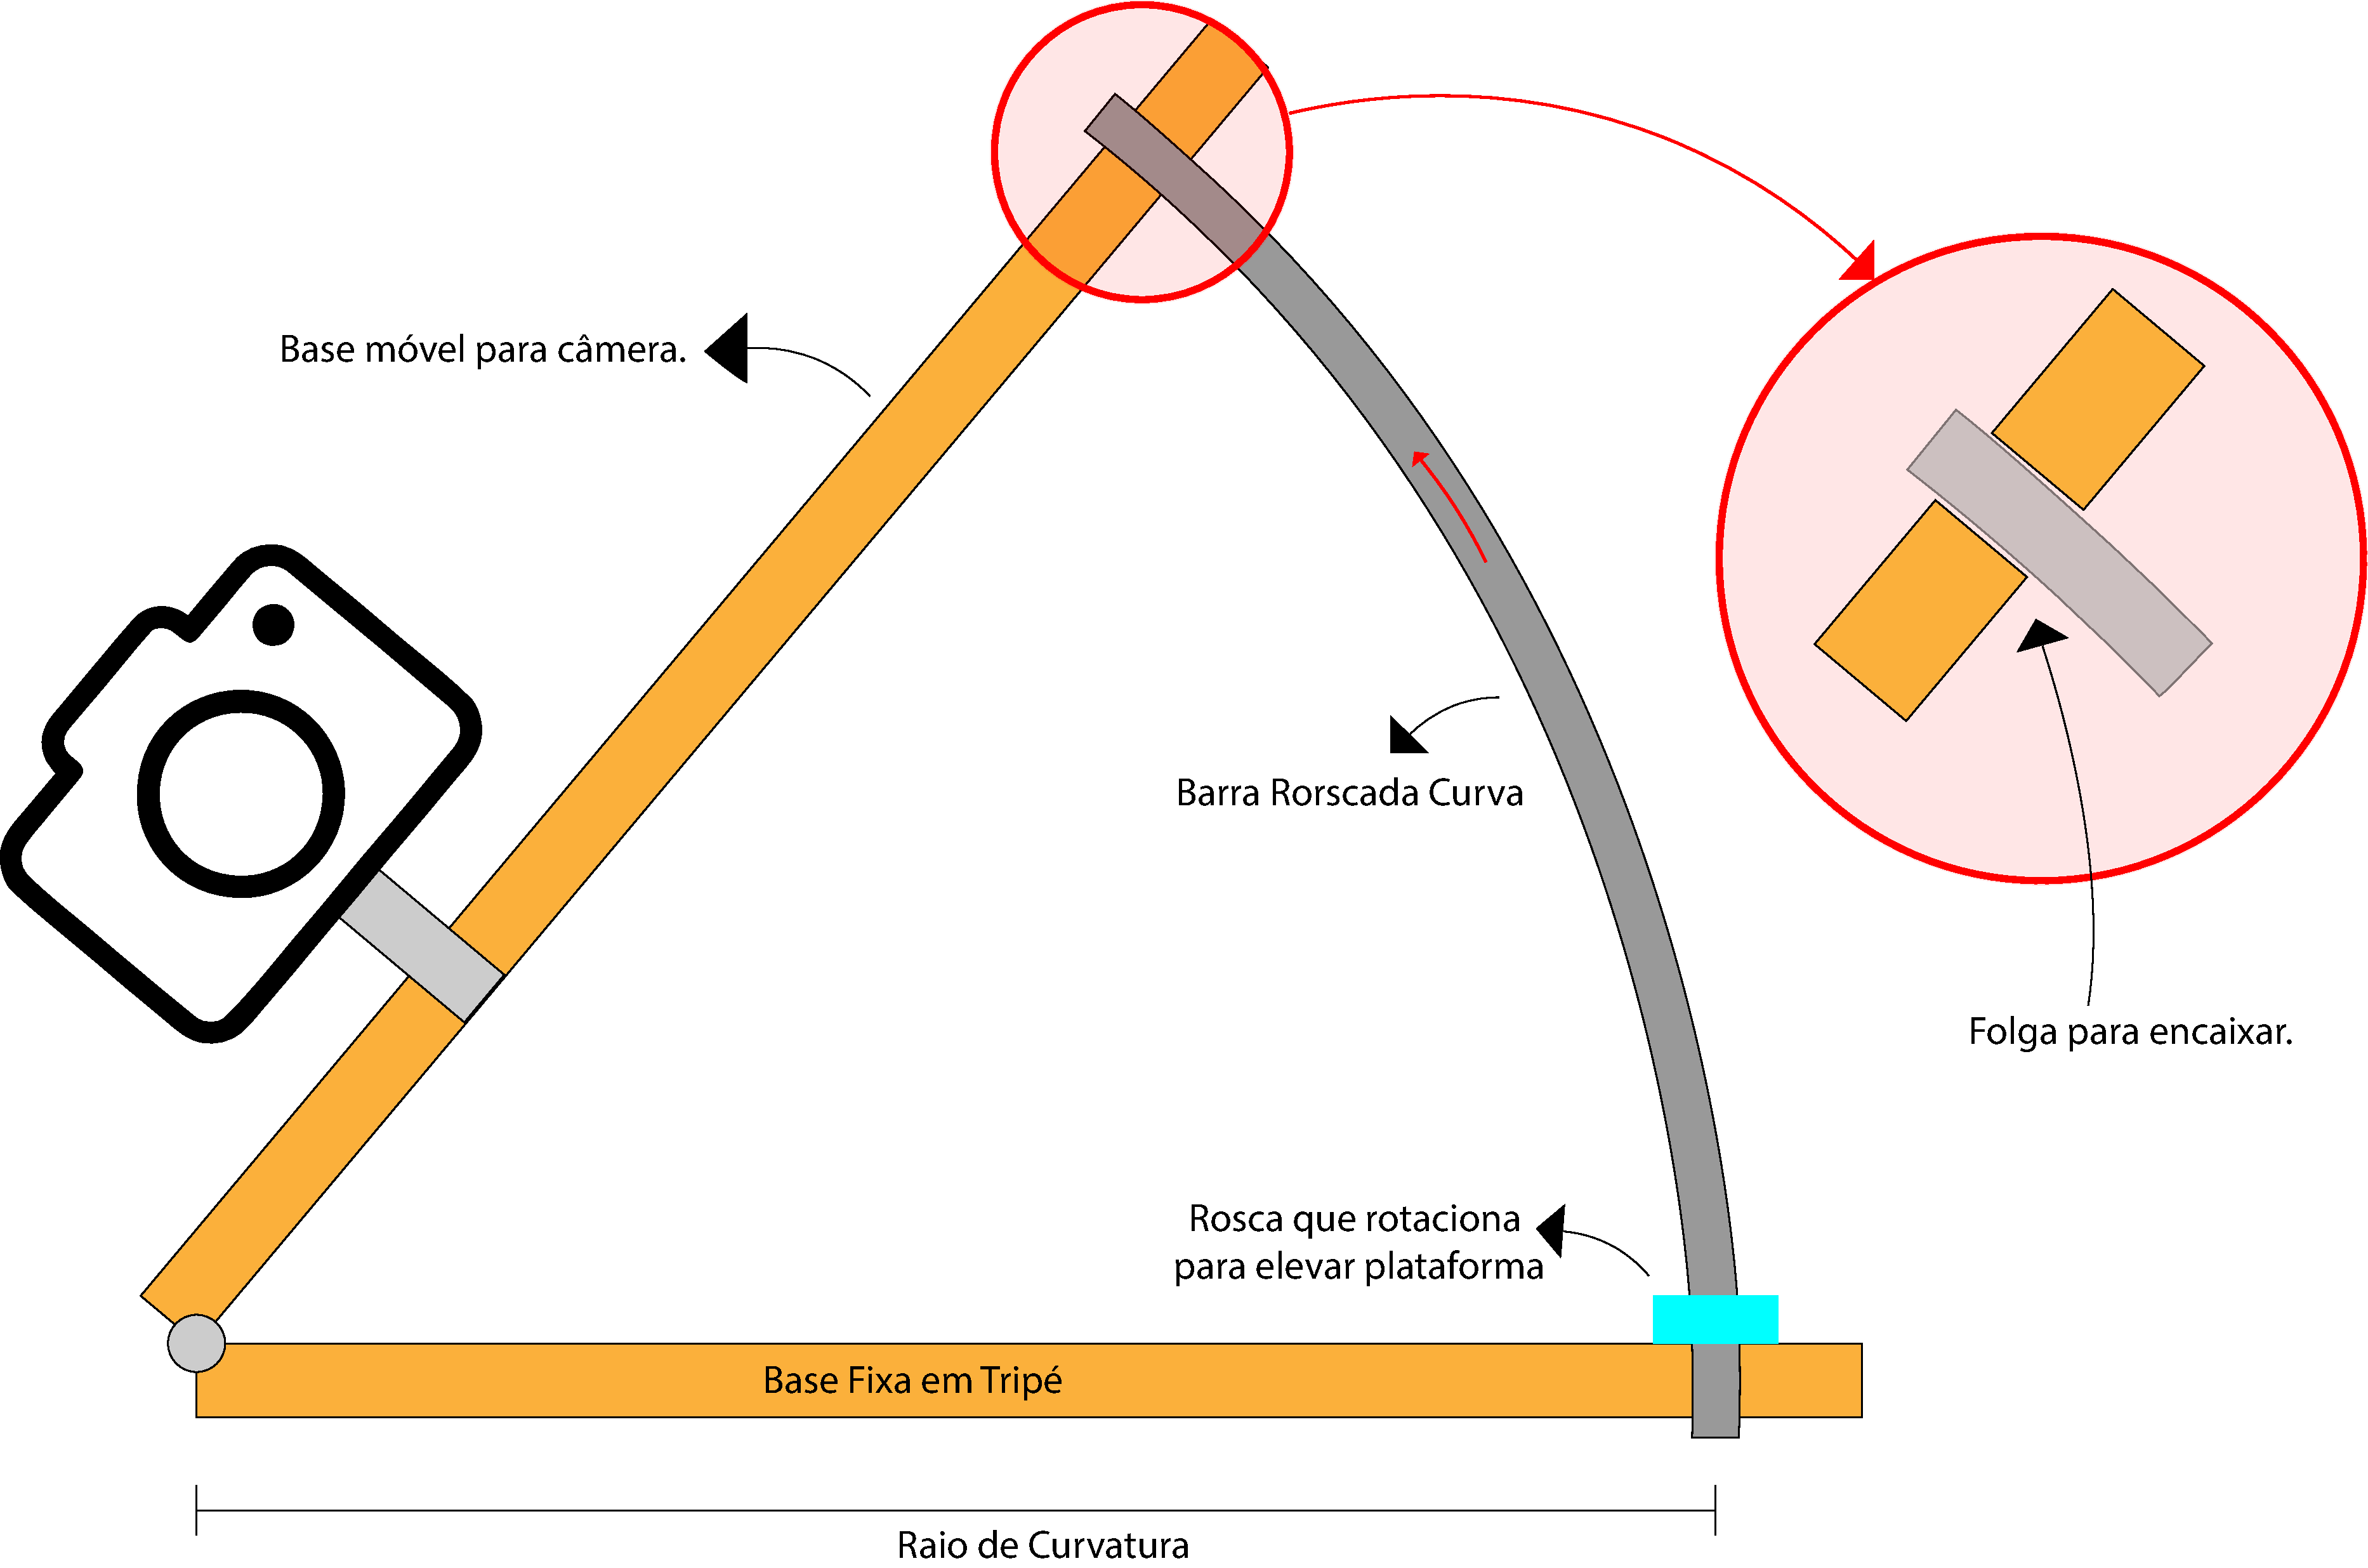
\includegraphics[width=0.6\linewidth]{figuras/revisaobiblio/montagemCurva}
 	\label{fig:montagemCurva}
 	\fonte{Adaptado de \cite{artigo:edjonescurved}.}
 \end{figure}

Comparando os atributos dos modelos de \textit{Barn Door}, a montagem curva é a mais apropriada para o projeto proposto, visto que não demanda a construção de um mecanismo demasiadamente complexo. Dessa forma, ela reduz a quantidade de materiais e processos, bem como a lógica de controle do motor, minimizando ainda mais os custos, ao passo que potencializa o resultado do projeto. 

\subsection{Métodos de Alinhamento Polar}
O alinhamento com o polo norte/sul celeste é fundamental para a execução da astrofotografia através de uma plataforma equatorial, e erros podem comprometer o funcionamento do sistema. Quanto mais bem alinhada está a plataforma, maior será o tempo de exposição que ela conseguirá obter sem gerar rastros nas estrelas. Para realizar esse alinhamento, existem dois métodos: Localizar a estrela Polar que indica a posição do polo celeste e/ou utilizar de instrumentação para posicionar a plataforma nos valores de azimute e inclinação corretos, dada a posição da plataforma no planeta.

\subsubsection{Localização da Estrela Polar}
Existem duas formas de alinhamento por meio da localização no céu da estrela polar. A primeira delas é um \textit{laser}, que é alinhado com a estrela polar para indicar o alinhamento (Figura \ref{fig:alinhamentolaser}). No entanto, o \textit{laser} não é um método extremamente confiável, pois a estrela polar não é exatamente centrada no polo norte celeste, dessa forma o alinhamento não fica preciso. As principais vantagens desse método são a facilidade e o baixo custo que é, em média, na ordem de US\$ 100.\footnote{Considerando modelos pesquisados em agosto de 2021}

% usar tudo em dollar
 \begin{figure}[!htb]
	\centering
	\caption{Alinhamento por \textit{laser}}
	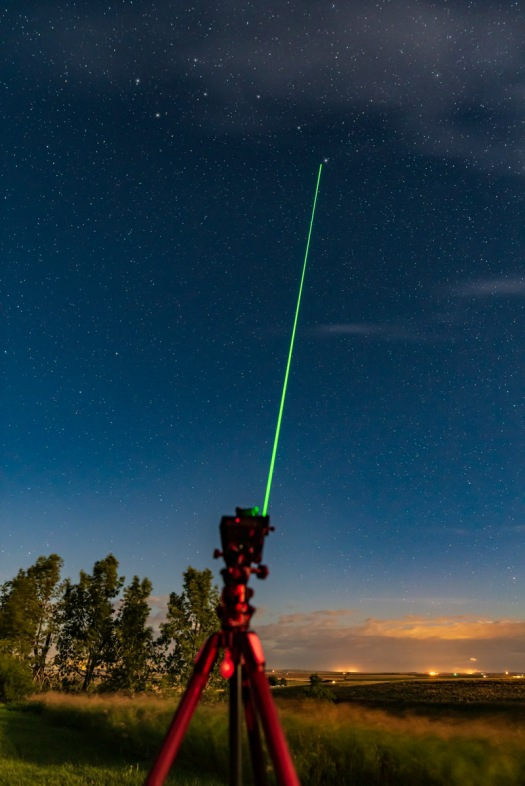
\includegraphics[width=0.3\linewidth]{figuras/revisaobiblio/alinhamentolaser}
	\label{fig:alinhamentolaser}
	\fonte{\cite{site:testingMSM}.}
\end{figure}


O segundo método envolve uma luneta que permita a identificação das constelações que indicam o polo Norte/Sul (Figura \ref{fig:luneta}). No hemisfério Norte, procura-se a estrela Polaris; no hemisfério Sul, busca-se a constelação de Sigma Octantis e o Cruzeiro do Sul. Ele é um método bem confiável, porém, no hemisfério Sul, isso normalmente é mais difícil, pois essas constelações são de alta magnitude. Isso significa dizer que possuem um baixo brilho, tornando-as difíceis de serem localizadas no céu. As lunetas buscadoras têm um custo bem variado, mas são normalmente comercializadas fora do Brasil e tem um custo que começa na casa dos US\$ 80 .\footnote{Considerando modelos pesquisados em agosto de 2021}

 \begin{figure}[!htb]
	\centering
	\caption{Visor de uma luneta para astrofotografia, contendo marcadores para alinhar as estrelas}
	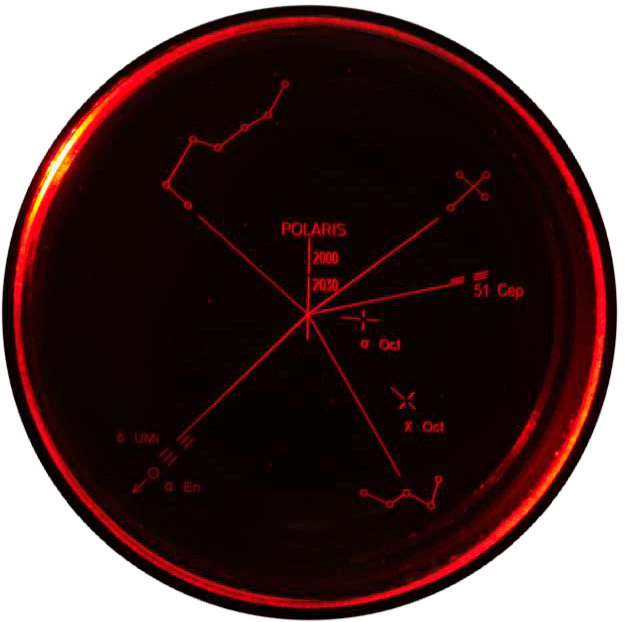
\includegraphics[width=0.5\linewidth]{figuras/revisaobiblio/luneta}
	\label{fig:luneta}
	\fonte{Adaptado de \cite{site:bresserpolarscope}.}
\end{figure}

Ambos os métodos possuem a desvantagem de requerer um céu limpo na região polar (Figura \ref{fig:temporuim}) e baixos níveis de poluição luminosa para identificar as estrelas, porém, apresentam a simplicidade como vantagem. O \textit{laser} é o menos confiável, pois existe uma defasagem entre as constelações e o polo celeste, que só é possível de ser compensado com o uso da luneta. 

 \begin{figure}[!htb]
	\centering
	\caption{Alinhamento impossível sem colaboração do tempo limpo}
	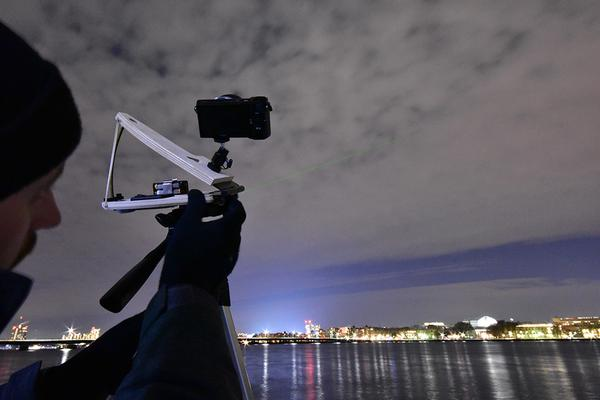
\includegraphics[width=0.5\linewidth]{figuras/revisaobiblio/temporuim}
	\label{fig:temporuim}
	\fonte{\cite{site:nyxtechtips}.}
\end{figure}


\subsubsection{Instrumentação}

Através de instrumentos de medição, é possível realizar o alinhamento da plataforma equatorial separando o processo em duas etapas. Na primeira etapa é feito o ajuste do azimute para alinhar a plataforma com o polo norte geográfico. Posteriormente, ela deve ser inclinada até o ângulo referente ao polo norte celeste que é dado pelo ângulo da latitude do local onde a plataforma está localizada, realizando um ajuste de elevação. 

\paragraph{Ajuste de Azimute}
O ajuste do azimute pode ser realizado com uma bússola ou um magnetômetro que possibilite indicar o polo norte magnético. No entanto, o polo norte geográfico possui uma diferença com o polo norte magnético devido à oscilação do campo magnético do planeta. Essa discrepância é chamada de declinação magnética. 

Além disso, devido à inconsistência do campo magnético, o valor da declinação é diferente para cada localização do planeta, mas pode ser calculada usando modelos magnéticos globais que são o resultado de pesquisas com sensores em satélites e apresentam valores com acurácia de 0,5 graus \cite{site:noicDecMag}.

\paragraph{Ajuste de Elevação}
O ajuste de elevação para uma determinada latitude pode ser feito através de marcações de ângulo em um eixo ou transformador (Figura \ref{fig:marcacao_latitude}), ou com sensores de posição inercial (acelerômetro e giroscópio) \cite{site:driftLupus}. É evidente que o primeiro método não é preciso, pois depende obrigatoriamente de um bom processo de manufatura e calibração, além da falta de precisão para ângulos de latitude com valores decimais. 

\begin{figure}[!htb]
	\centering
	\caption{Marcação da latitude para ajuste de elevação}
	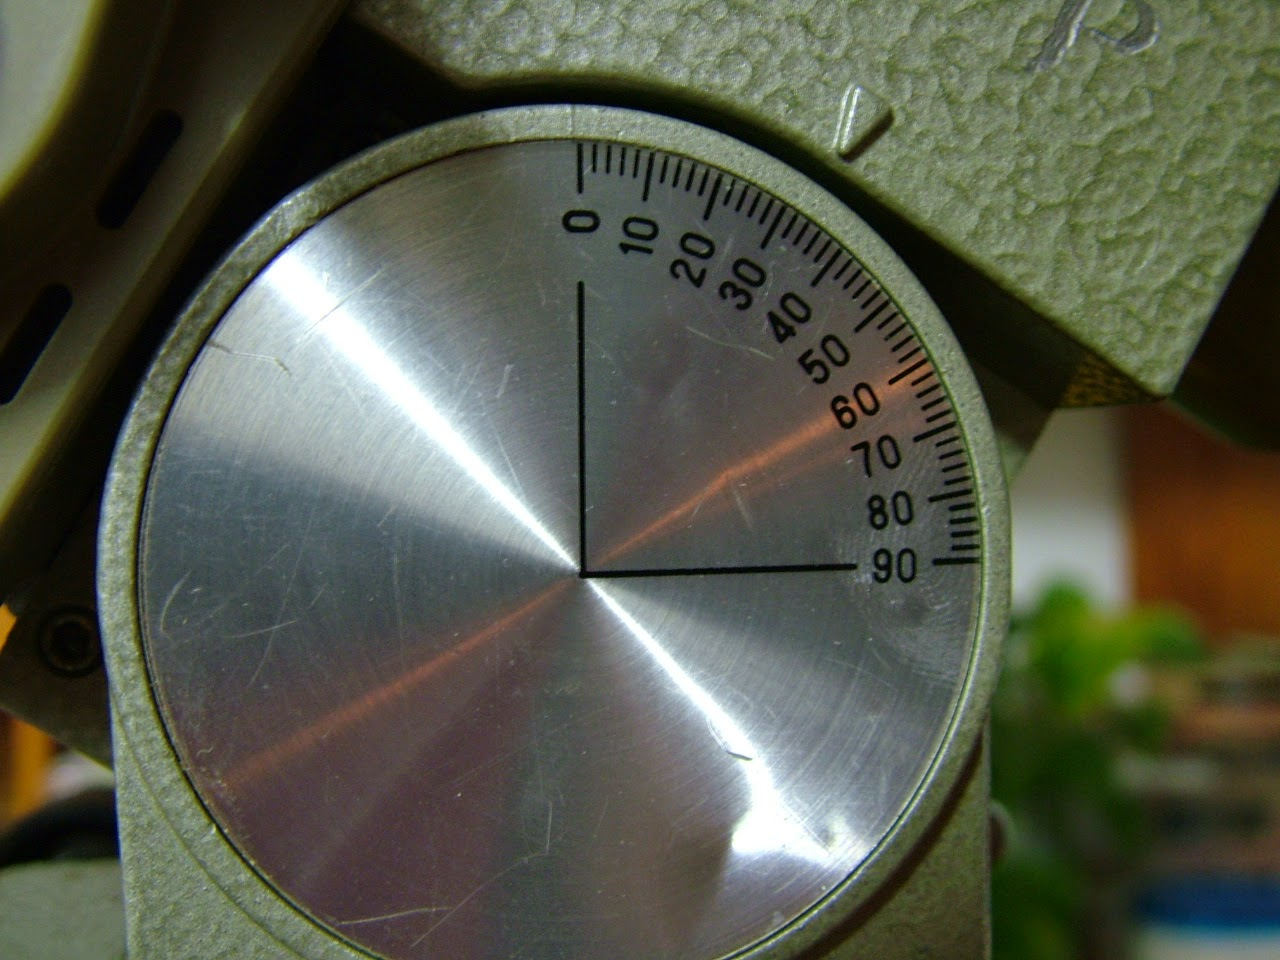
\includegraphics[width=0.45\linewidth]{figuras/revisaobiblio/marcacao_latitude}
	\label{fig:marcacao_latitude}
	\fonte{\cite{site:driftLupus}.}
\end{figure}

\subsubsection{Método \textit{Drift}}

O alinhamento da plataforma com o polo celeste é fundamental para uma longa exposição usando uma lente com grande comprimento focal. Se a montagem não estiver corretamente alinhada, ela não irá conseguir impedir o surgimento de rastro na fotografia por um longo período de tempo \cite{book:bbcsky}.  

Plataformas que são alinhadas com uma luneta polar conseguem atingir normalmente 180s de exposição. Se mais tempo for necessário ou for usada uma lente com muita ampliação, então o método \textit{Drift} de alinhamento é mandatório, ainda que, não é possível realizar esse ajuste de precisão sem que a plataforma já tenha sido previamente alinhada \cite{book:bbcsky}. 

O método consiste em localizar, primeiramente, uma estrela brilhante o suficiente para visualizar no visor da câmera, e que esteja na linha do equador polar. Habilitando uma linha de grade no visor, o usuário deve alinhar a estrela escolhida de forma que fique centralizada no cruzamento da grelha (Figura \ref{fig:driftgrelha1}) e, então, ligar o rastreador, observando se haverá movimentação da estrela para algum dos lados do visor. Na sequência, o usuário deve apontar para uma estrela ao leste ou oeste, no horizonte, e observar para qual lado (esquerda/direita ou Norte/Sul) do visor haverá fuga (Figura \ref{fig:driftgrelha2}). O lado (esquerda ou direita) que indica Norte ou Sul depende para onde a câmera estiver sendo apontada e a orientação dela \cite{book:bbcsky}.

\begin{figure}[hbt]
	\centering
	\caption{Estrela centralizada na grelha do visor da câmera}
	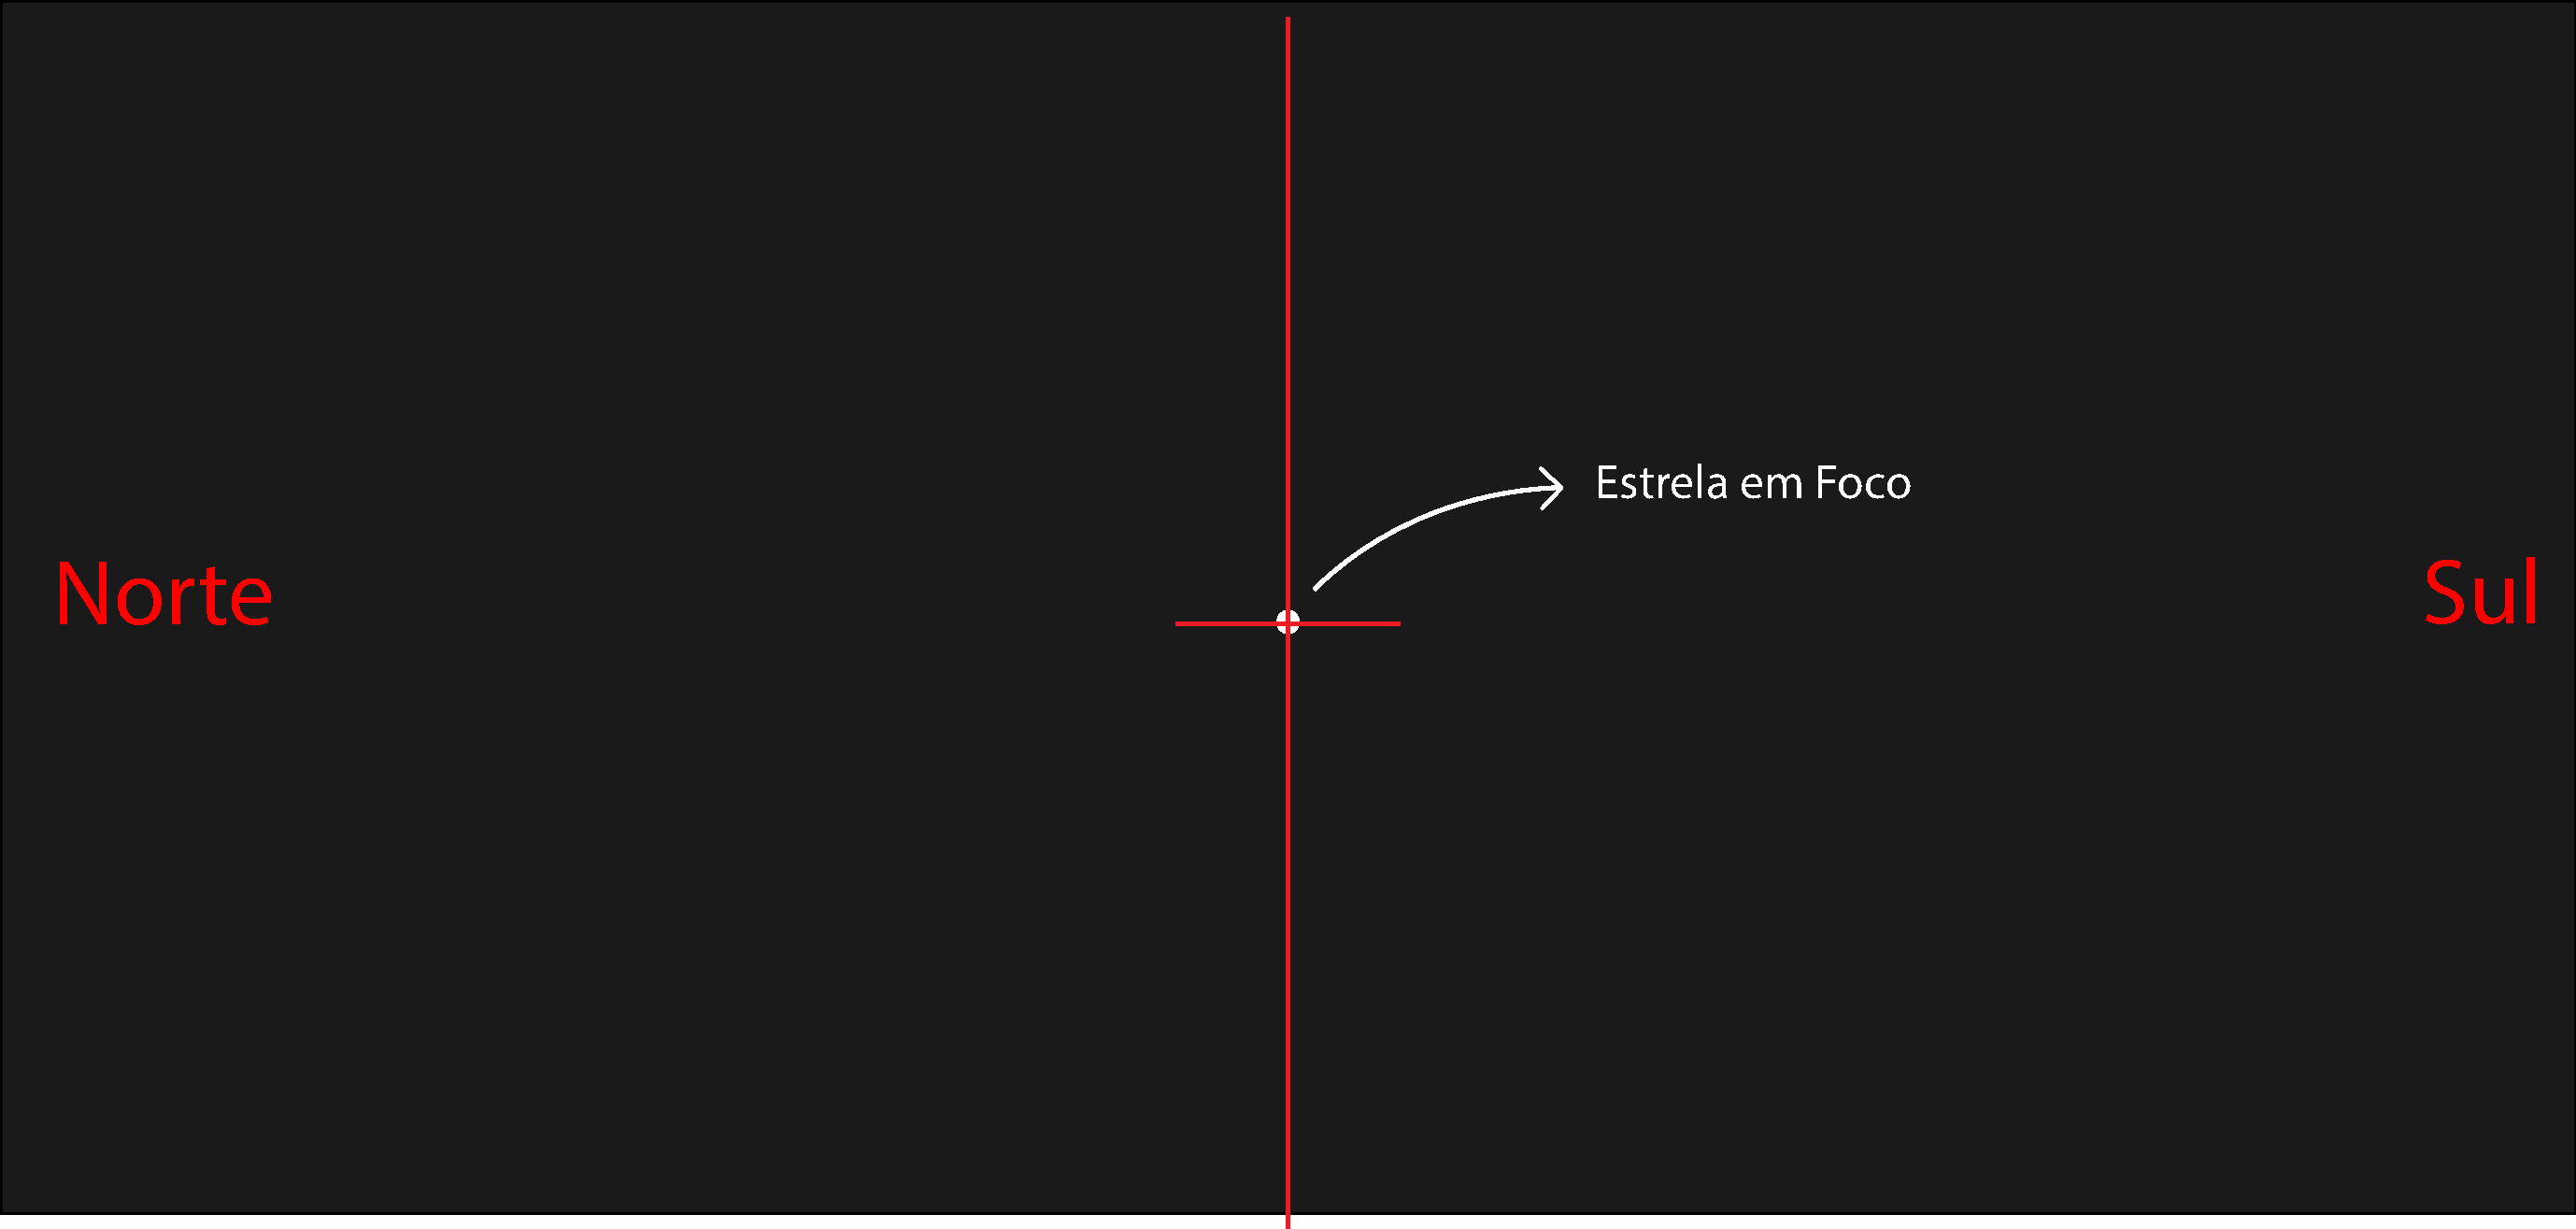
\includegraphics[width=0.7\linewidth]{figuras/revisaobiblio/driftgrelha1}
	\label{fig:driftgrelha1}
	\fonte{Adaptado de \cite{site:driftLupus}.}
\end{figure}

\begin{figure}[hbt]
	\centering
	\caption{Estrela apresentando fuga para a direita que, neste caso, aponta para o Sul}
	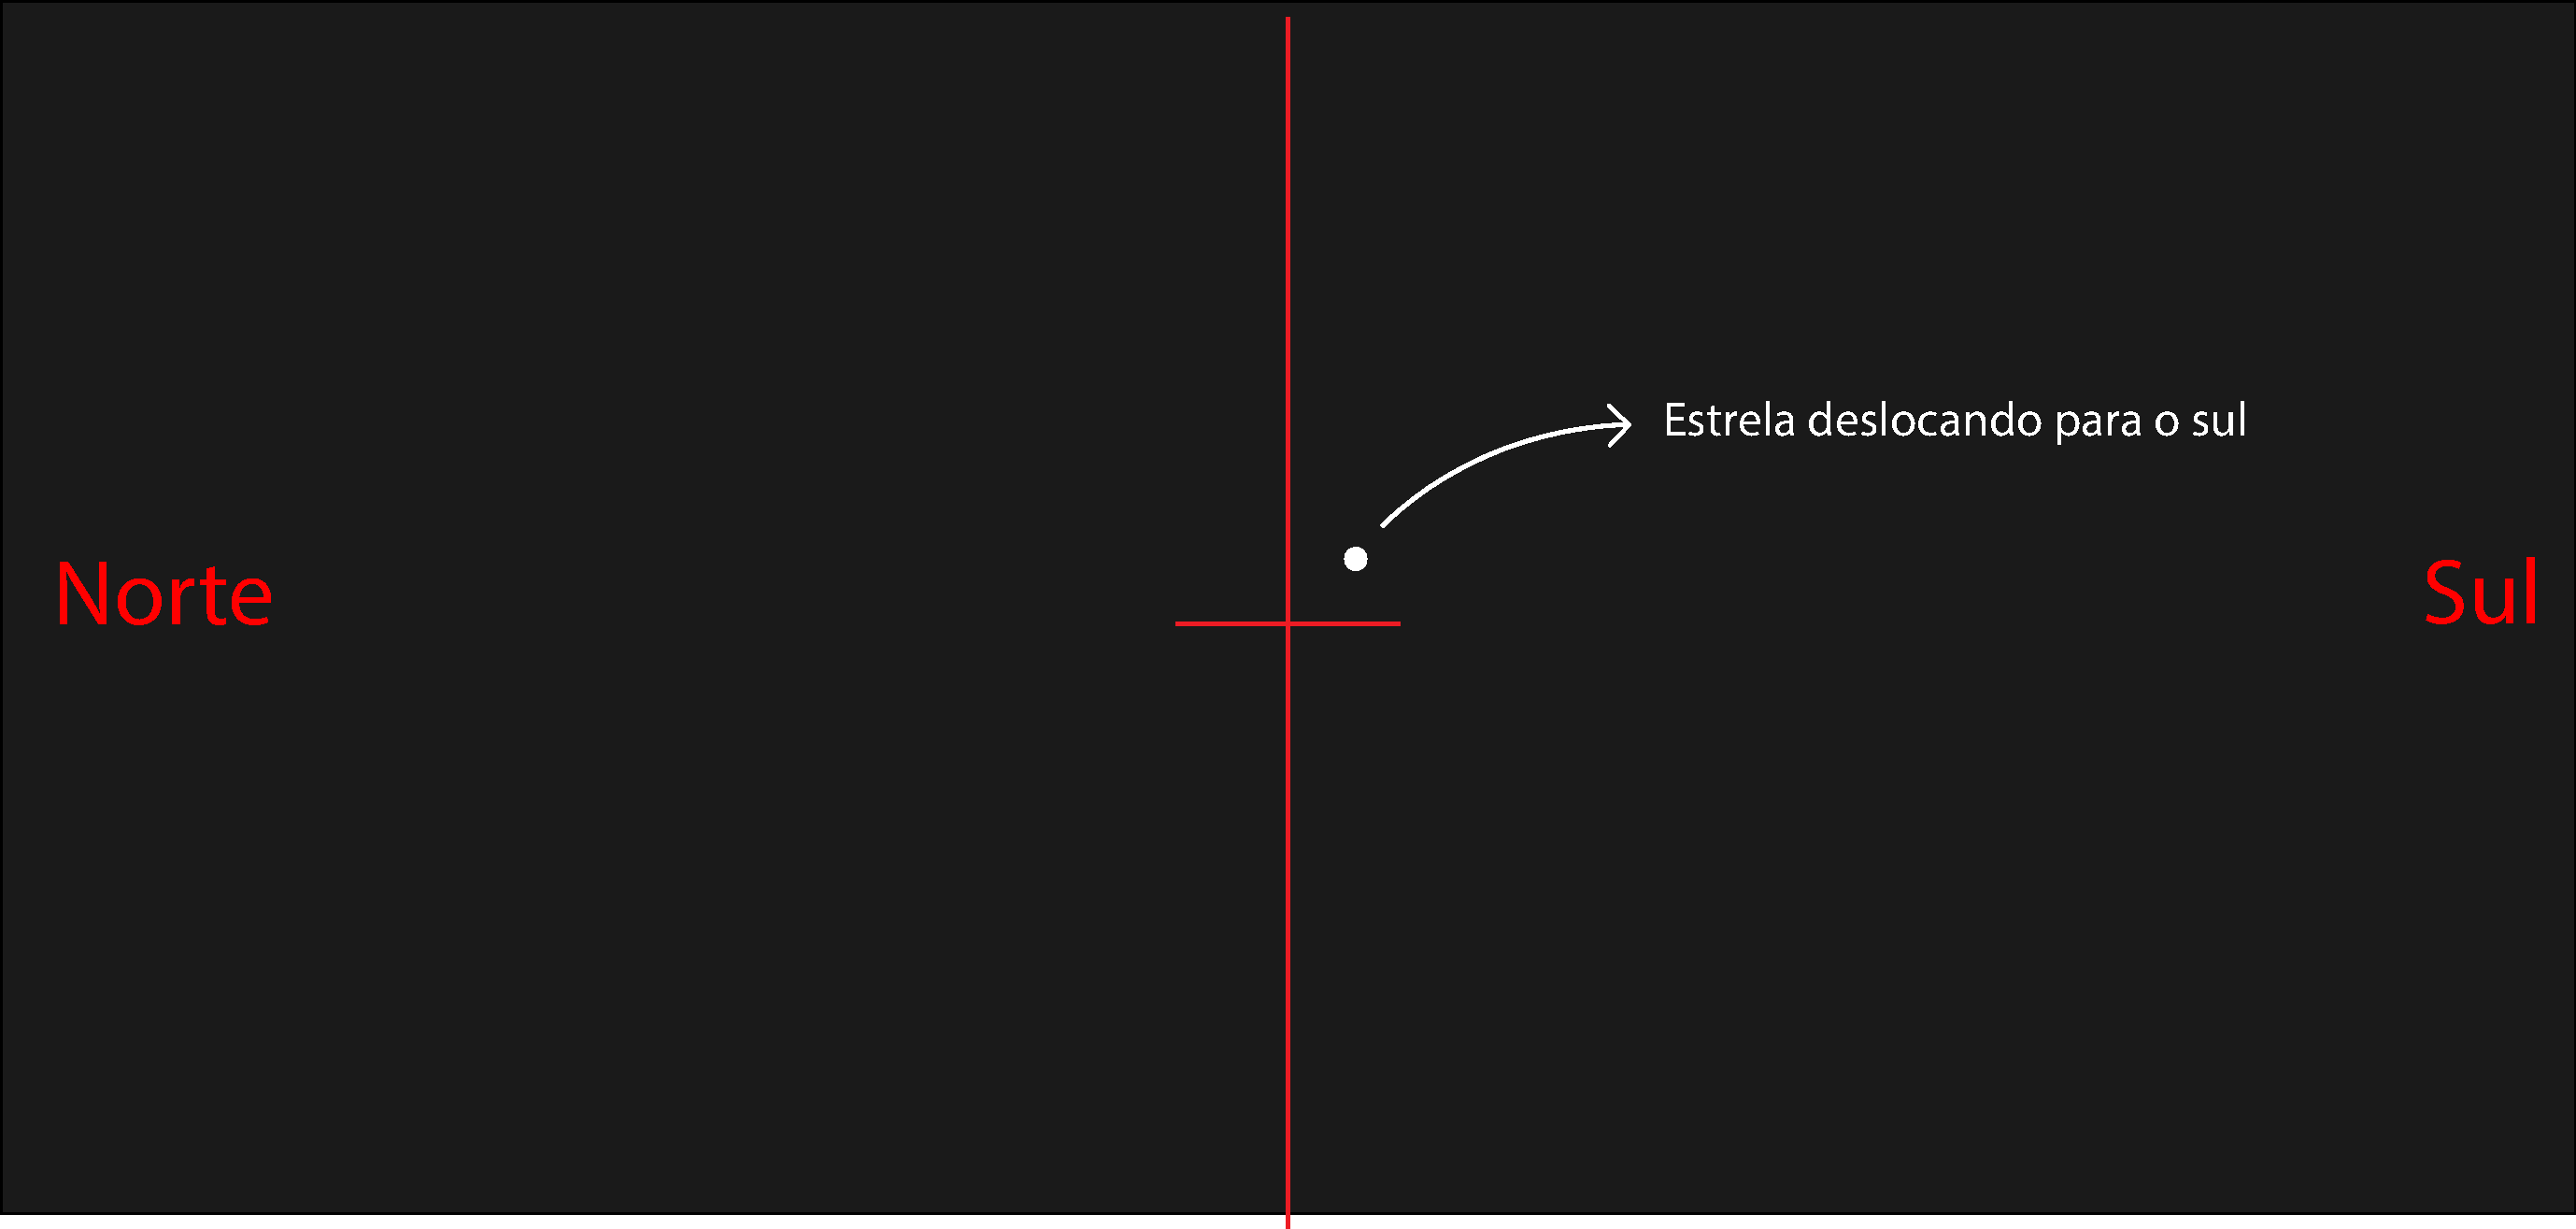
\includegraphics[width=0.7\linewidth]{figuras/revisaobiblio/driftgrelha2}
	\label{fig:driftgrelha2}
	\fonte{Adaptado de \cite{site:driftLupus}.}
\end{figure}

Dependendo para qual lado do visor (norte/sul) houver fuga, deverá ser feito um ajuste específico no alinhamento, que também é diferente para cada hemisfério do planeta. O fotógrafo deve saber para qual lado do visor é norte ou sul, pois será isso que determinará corretamente a correção para movimentar a plataforma (Tabela \ref{tab:drift}). A primeira estrela ajuda a ajustar o azimute da plataforma e a segunda colabora para uma elevação correta. Além disso, a precisão do ajuste dependerá do tempo que a estrela irá levar para sair da marcação do visor, e o processo de repete até que a estrela permaneça parada pelo tempo mínimo desejado pelo fotógrafo para a lente que estiver usando \cite{book:bbcsky}. 

\begin{table}[!htp]
	\centering
	\caption{Ajustes do método \textit{Drift} para cada caso}
	\label{tab:drift}		
		\begin{tabular}{c|c|c|c}
			\makecell{Localização\\da estrela} & Lado da Fuga & \makecell{Correção\\(Hemisfério Sul)}& \makecell{Correção\\(Hemisfério Norte)}\\  \hline
			\multirow{2}{*}{ Meridiano } & Norte & Azimute para Leste & Azimute para Leste \\ \cline{2-4}
			& Sul & Azimute para Oeste & Azimute para Oeste \\ \hline
			\multirow{2}{*}{ Leste } & Norte & Altura para cima & Altura para baixo \\ \cline{2-4}
			& Sul & Altura para baixo & Altura para cima \\ \hline
			\multirow{2}{*}{ Oeste } & Norte & Altura para baixo & Altura para cima \\ \cline{2-4}
			& Sul & Altura para cima & Altura para baixo \\ 
		\end{tabular}
	
	\fonte{Adaptado de \cite{site:driftLupus}.}
\end{table}

É importante ressaltar que para esse método ser possível, o tripé onde a plataforma é montada deve possuir \textit{knobs} para ajuste mais acurado, como na cabeça de tripé da Figura \ref{fig:ballhead}, que possui um \textit{knob} para movimentação somente de azimute, outro para movimento livre, e um terceiro para um ajuste mais preciso de ambas as posições. Além dessa, existem cabeças para filmagem que permitem um controle ainda mais suave e preciso, sendo extremamente recomendadas para esse método (Figura \ref{fig:ballheadfilmagem}).

\begin{figure}[!htb]
	\centering
	\caption{Cabeça de Tripé com possibilidade para ajuste de precisão}
	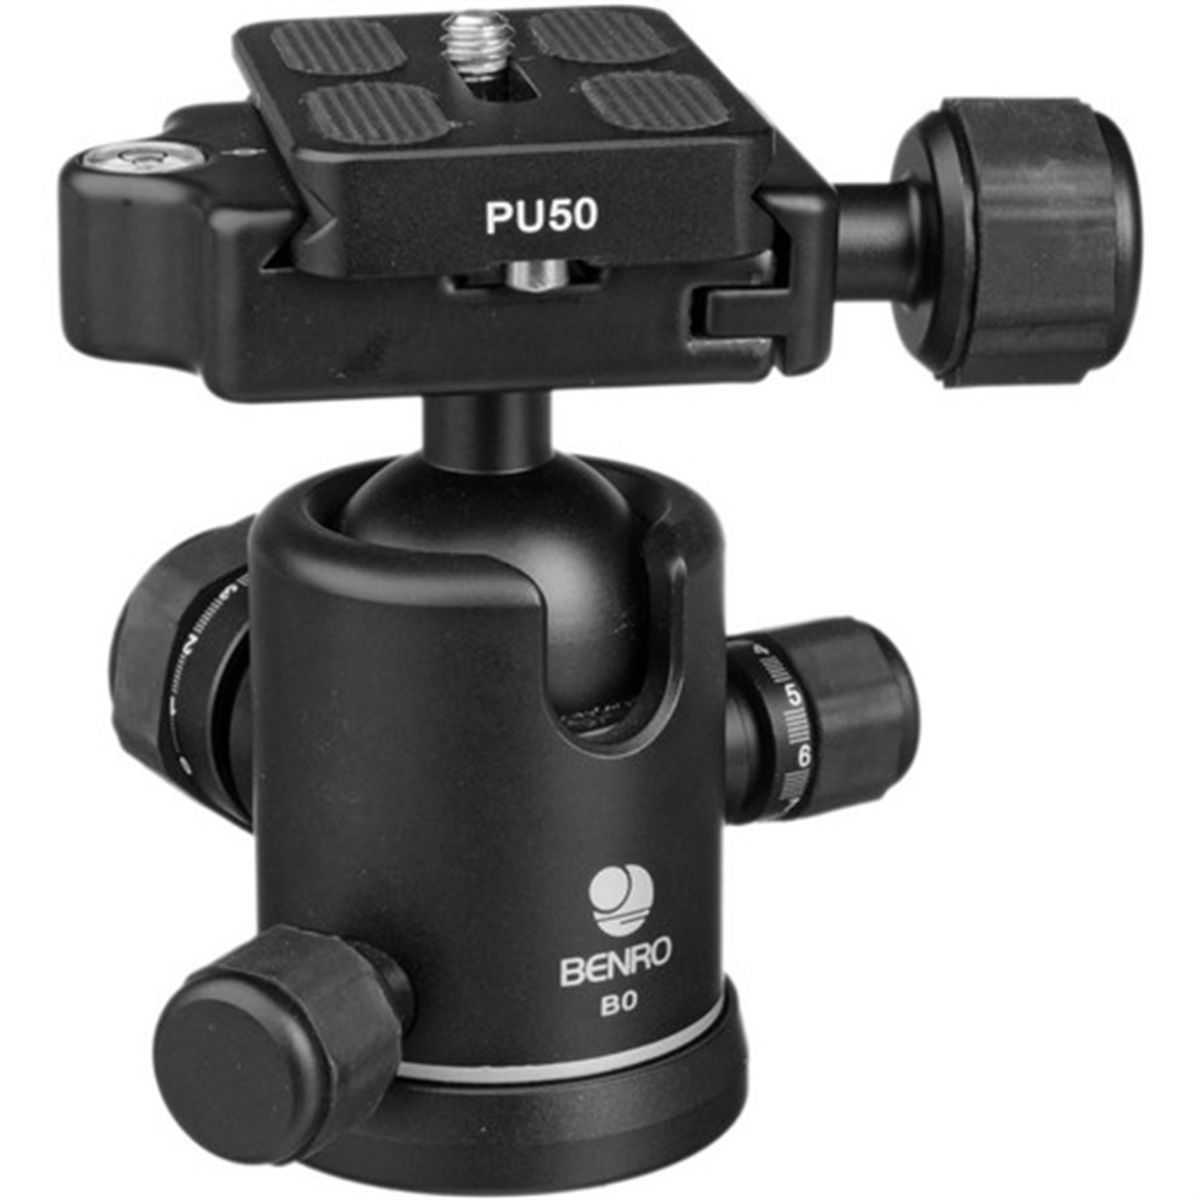
\includegraphics[width=0.3\linewidth]{figuras/revisaobiblio/ballhead}
	\label{fig:ballhead}
	\fonte{(Optison, c2021).}
\end{figure}

\begin{figure}[!htb]
	\centering
	\caption{Cabeça de Tripé com possibilidade para ajuste de precisão}
	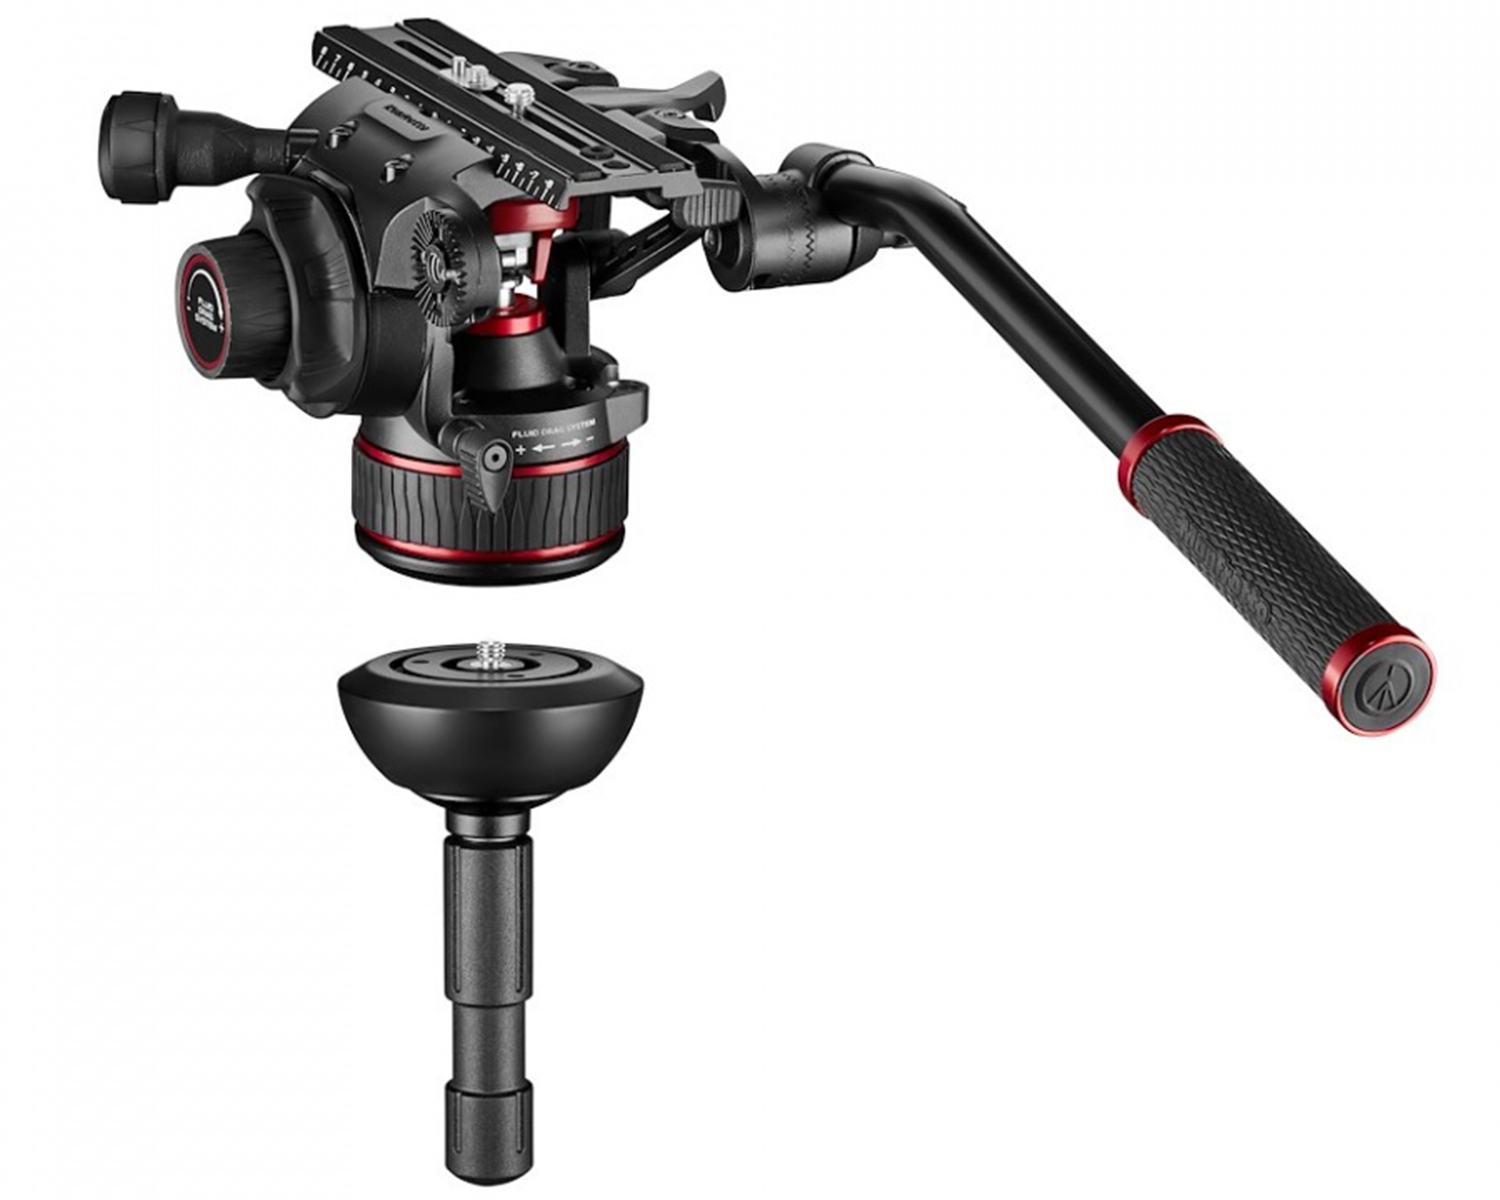
\includegraphics[width=0.4\linewidth]{figuras/revisaobiblio/video-head}
	\label{fig:ballheadfilmagem}
	\fonte{(Manfrotto, c2021).}
\end{figure}

\subsection{Soluções Comerciais Existentes}

Existem inúmeras soluções comerciais para o problema proposto, porém, todos usam uma luneta ou um \textit{laser} como método de alinhamento polar. Existem produtos com diferentes especificações e orçamentos. A Tabela \ref{tabela_benchmark} ilustra alguns sistemas, dentre os disponíveis no mercado, comparando suas funcionalidades. 


\begin{table}[htb]
	\caption{Comparativo das Soluções de Mercado}
	\begin{tabular}{l|cccc}
		& Nyx Tracker & iOptron & Vixen Optics & SkyWatcher \\ \hline
		Preço (US\$) & 115 & 299 & 399 & 299 \\\hline
		Carga Máxima (kg) & 2.25 & 3 & 2 & 3 \\\hline
		Erro periódico (arcsec) & 115 & 100 & 50 & 50 \\\hline
		Volume (cm$^2$) & 155 & 490 & 323 & 220 \\\hline
		Peso (kg) & 0,4 & 1,15 & 0,79 & 0,72 \\\hline
		Alinhamento & \textit{Laser} & \textit{Polar Scope} & \textit{Polar Scope} & \textit{Polar Scope} \\
	\end{tabular}
	\label{tabela_benchmark}
	\fonte{Adaptado de \cite{site:nyxtech}.}
\end{table}

Contudo, na realidade brasileira, o preço mostrado passaria ainda por impostos, tornando a compra mais inviável. O Nyx Tracker (Figura \ref{fig:nyxtracker}) é o único da lista que possui uma estrutura de \textit{Barn Door}, e é o sistema mais acessível, porém o método de alinhamento é de difícil execução no hemisfério sul.

\begin{figure}[h]
	\centering
	\caption{Nyx Tracker}
	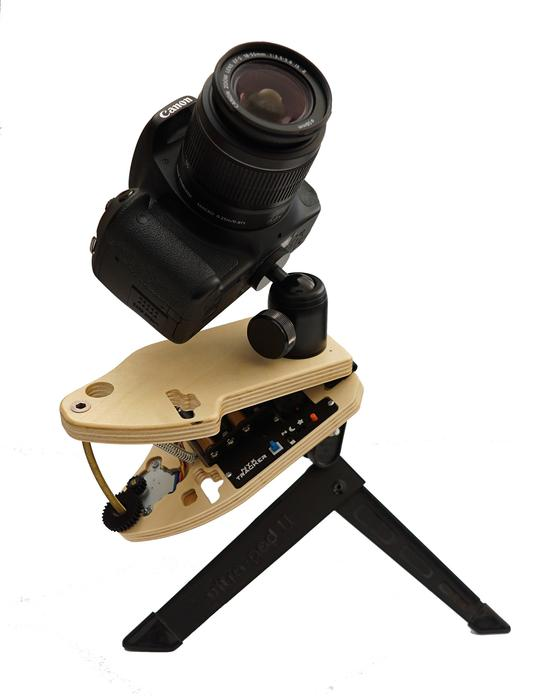
\includegraphics[width=0.3\linewidth]{figuras/revisaobiblio/nyxtracker}
	\label{fig:nyxtracker}
	\fonte{\cite{site:nyxtech}.}
\end{figure}


\section{Objetivos}

Pelo \textit{benchmark} exposto, fixaram-se como objetivos o desenvolvimento de uma solução robusta, visualmente elegante, e que consiga se aproximar das propriedades do modelo comercial mais acessível, com o custo inferior a US\$115 . Além disso, deve ter como diferencial um aplicativo que permita uma fácil interação do usuário com o sistema, facilitando o processo de configuração e alinhamento polar.

\section{Sistemas Embarcados}

Um sistema embarcado é definido como um conjunto de periféricos controlados por um microcontrolador ou microprocessador (Figura \ref{fig:embbedsystem}) de uma forma oculta ao usuário final. O "cérebro" funciona por meio de um \textit{software}, que é um conjunto de instruções elaborado por um programador e é executado em \textit{hardware} \cite{book:ANSIC}.

\begin{figure}[!htb]
	\centering
	\caption{Visualização conceitual de um sistema embarcado.}
	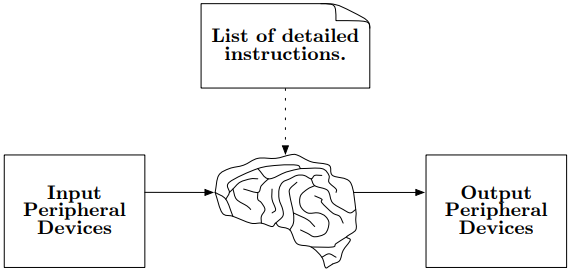
\includegraphics[width=0.7\linewidth]{figuras/revisaobiblio/embbedsystem}
	\label{fig:embbedsystem}
	\fonte{Adaptado de \cite{book:ANSIC}.}
\end{figure}

Os periféricos são o conjunto de dispositivos conectados ao controlador para executar uma leitura de dados ou ação externa. Sensores, botões e interfaces são exemplos de dispositivos periféricos para leitura de dados. Motores, LEDs e atuadores lineares são exemplos que executam uma ação ordenada. As conexões destes periféricos com os controladores são construídas por meio de condutores e semicondutores como resistores, capacitores, transistores, diodos, etc. \cite{book:ANSIC}. 


\section{Periféricos}

No contexto do projeto, propõe-se um sistema embarcado que utiliza sensores para realizar a leitura da posição geográfica e inercial da plataforma equatorial, e guiar o usuário na sua configuração. Após esse ajuste, o usuário pode ativar um atuador que irá realizar o rastreamento do movimento aparente das estrelas no céu. 

Dessa forma, é necessário a leitura de Sensores de Posição Inercia (IMU) e um sinal de GPS (Sistema de Posicionamento Global). É preciso também um motor de passo que servirá como o atuador da plataforma.

\subsection{Motor de Passo}

O motor de passo é um tipo de atuador comumente utilizado em aplicações de controle, como impressoras 3D, máquinas CNC, entre outros sistemas que requerem uma boa precisão. Além disso, os motores de passo também possuem outros pontos fortes: não tem escovas internas que podem gerar curto circuito; não são dependentes da carga aplicada, mantendo a velocidade de rotação constante desde que o torque necessário não exceda os limites; giram em passos que são incrementados de forma constante durante a sua aplicação, possibilitando um controle preciso sem a necessidade de um sensor com \textit{feedback}; e, por fim, conseguem manter o sistema imóvel quando estacionados \cite{manual:stepperMicrochip}.

Existem dois tipos mais comuns de motores de passo (Figura \ref{fig:stepper_polar}): unipolar e bipolar, que se diferenciam pela forma em que as bobinas são conectadas e energizadas para movimentar o rotor. No motor unipolar, cada bobina é controlada individualmente; no motor bipolar, as bobinas são agrupadas e controladas em conjunto para ganhar desempenho. \cite{man:advancedmicrosystemStepControl}.

\begin{figure}[!htb]
	\centering
	\captionsetup[subfigure]{justification=centering}
	\caption{Modelos de motores: (a) um motor unipolar, (b) motor bipolar}
	\begin{subfigure}[b]{0.49\textwidth}
		\centering
		\includegraphics[width=.6\textwidth]{figuras/revisaobiblio/stepper_polar_a}
		\caption{}
		\label{fig:stepper_polara}
	\end{subfigure}
	\hfill
	\begin{subfigure}[b]{0.49\textwidth}
		\centering
		\includegraphics[width=.6\textwidth]{figuras/revisaobiblio/stepper_polar_b}
		\caption{}
		\label{fig:stepper_polarb}
	\end{subfigure}

\label{fig:stepper_polar}
	\fonte{Adaptado de \cite{man:advancedmicrosystemStepControl}.}
\end{figure}

\subsubsection{Driver}

Para que a corrente flua pelas bobinas e seja controlada por um controlador, é preciso um \textit{driver} que realize o chaveamento pois, normalmente, microcontroladores não conseguem fornecer corrente para energizar um motor de passo. Os \textit{drivers} são circuitos integrados com transistores e atendem ao princípio de funcionamento dos tipos de motores. O diagrama do controle de um motor pode ser simplificado como demonstra a Figura \ref{fig:connectionstepper}, onde o microcontrolador -após receber um sinal da máquina, ou de um usuário- atua em um \textit{driver}, enviando pulsos pelas suas saídas. O driver recebe esses sinais e atua diretamente no motor, liberando corrente e operando a máquina.

\begin{figure}[!htb]
	\centering
	\caption{Diagrama de controle de um motor de passo}
	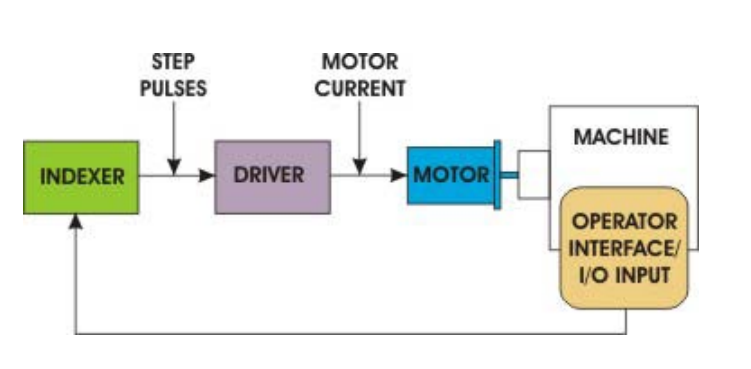
\includegraphics[width=.7\linewidth]{figuras/revisaobiblio/connectionstepper}
	\label{fig:connectionstepper}
	\fonte{Adaptado de \cite{man:advancedmicrosystemStepControl}.}
\end{figure}

\subsubsection{Torque}

Torque é o momento da força que um motor consegue aplicar no seu eixo de rotação. Normalmente, motores de passo tem diferentes valores de torque que os caracterizam para cada situação de aplicação e são descritos pelos fabricantes \cite{manual:stepperMicrochip}. Além disso, é preciso manter-se atento ao consumo necessário: quanto maior o torque exigido do motor, maior será a corrente que ele irá demandar sob a carga aplicada. Têm-se os seguintes tipos de torque em motores de passo. 

\begin{itemize}
	\item \textit{Holding torque} – Torque mínimo para girar o eixo do motor enquanto os enrolamentos são energizados.
	
	\item \textit{Detent torque} – Torque necessário para tirar o eixo da inércia quando os enrolamentos não são energizados.
	
	\item \textit{Pull-in torque} – Torque máximo suportado para iniciar a rotação dos eixos, sem perder passos, e em uma aceleração constante.
	
	\item \textit{Pull-out torque} – Torque máximo suportado quando o motor já estiver rotacionando em velocidade constante.

\end{itemize}

\subsubsection{Tamanho do Passo}
Cada sinal que é enviado ao motor faz com que o rotor gire um passo. Esse tamanho de passo é uma característica de cada atuador e define a resolução mínima de movimento angular que o eixo consegue realizar. Essa característica é importante pois quanto maior a precisão da aplicação, maior deve ser o número de passos no motor. Por exemplo, um motor que contenha 200 passos consegue ter uma precisão de $ 360^{\circ} \div 200 = 1,8 ^{\circ} $.

Apesar da precisão dos motores, é possível que ocorram erros ao rotacionar em cada passo. Esses problemas derivam de falhas mecânicas inerentes aos mecanismos internos do motor, não são cumulativas e oscilam de 3 a 5\% de erro no deslocamento \cite{man:advancedmicrosystemStepControl}.

\subsubsection{Formas de Controle}
Existem três diferentes abordagens para realizar o chaveamento das bobinas de um motor de passo: \textit{Full Step}, \textit{Half Step} e \textit{Microstep}. Essas técnicas são aplicáveis a qualquer tipo de motor.

\paragraph{Full Step}
Essa é a forma mais simples de controlar o motor: para cada pulso do controlador, uma bobina é ativada completamente e isso é alternado ao longo do tempo (Tabela \ref{tab:fs}). Nesse modo, o motor consome mais corrente, oferece mais torque e gera mais ruído. Além disso, considerando o exemplo de motor da seção anterior, com 200 passos, o controlador irá precisar emitir 200 pulsos no \textit{driver} para que o motor dê um giro de 360 graus \cite{man:advancedmicrosystemStepControl}.

\begin{table}[!htb]
	\centering
	\caption{Sequência de acionamentos das bobinas do motor pelo microcontrolador no modo \textit{Full Step}}
	\begin{tabular}{c|c|c|c|c}
		Passo & B.1 & B.2 & B.3 & B.4 \\\hline
		1	& 1 & 0 & 0 & 0\\
		2	& 0 & 1 & 0 & 0\\
		3	& 0 & 0 & 1 & 0\\
		4	& 0 & 0	& 0 & 1		\\
	\end{tabular}
	\label{tab:fs}
	\fonte{\cite{site:eletrogateguiamotor}.}
\end{table}


\paragraph{Half Step}
Um controle \textit{Half Step} proporciona uma redução no ruído e ganho de eficiência, porém reduz o torque máximo do motor. Essa abordagem funciona subdividindo as etapas de controle no modo \textit{Full Step}, consumindo 400 pulsos do controlador que acionam 2 bobinas para cada pulso, com um sinal intermediário acionando somente uma bobina (Tabela \ref{tab:hs}) \cite{man:advancedmicrosystemStepControl}.

\begin{table}[!htb]
	\centering	
	\caption{Sequência de acionamentos das bobinas do motor pelo microcontrolador no modo \textit{Half Step}}
	\begin{tabular}{c|c|c|c|c}
				Passo & B.1 & B.2 & B.3 & B.4 \\\hline
		1	& 1 & 0 & 0 & 0\\
		2	& 1 & 1 & 0 & 0\\
		3	& 0 & 1 & 0 & 0\\
		4	& 0 & 1	& 1 & 0\\
		5	& 0 & 0 & 1 & 0\\
		6	& 0 & 0 & 1 & 1\\
		7	& 0 & 0 & 0 & 1\\
		8	& 1 & 0	& 0 & 1\\
	\end{tabular}
	\label{tab:hs}
	\fonte{\cite{site:eletrogateguiamotor}.}
\end{table}

\paragraph{Microstep}
Uma abordagem de \textit{Microstep} busca suavizar ainda mais o controle do motor para reduzir o ruído e ganhar eficiência ao custo de perder torque. Esse método subdivide o controle em ainda mais etapas, requerindo \textit{drivers} especializados que podem energizar as bobinas de forma suave ao longo do tempo. 

\subsection{GPS}
O GPS (\textit{Global Positioning System}) é um sistema navegação por rádio que recebe informações via satélite para determinar a posição global de um objeto \cite{apostilagps}. Atualmente, todo \textit{Smartphone} ou aparelho celular contém um circuito capaz de realizar a leitura do sinal GPS e determinar sua localização atual. No entanto, a precisão da localização depende de um bom sinal dos satélites, podendo ter poucos metros de erro.

O valor retornado pelo GPS pode ser dado em coordenadas geográficas ou em UTM (\textit{Universal Transversa de Mercator}) que é um sistema de coordenadas planas. As coordenadas geográficas podem ser expressadas em: graus-minutos-segundos ($ ggg^o mm" ss,s"" $); graus-minutos-decimais ($ ggg^o mm,m" $); graus-decimais ($ ggg,g^o $) \cite{apostilagps}. 


\subsection{Sensores de Posição Inercial}

A posição de uma plataforma qualquer pode ser descrita por um sistema de coordenadas. Um padrão muito comum é o sistema RPY (\textit{Roll, Pitch, Yaw}) que expressa a posição por meio dos 3 ângulos posicionais do objeto (Figura \ref{fig:RPY}) \cite{diss:FabioAUV}. Os 3 ângulos são relativos a um dos 3 eixos \textit{x}, \textit{y} ou \textit{z} e podem ser traduzidos, respectivamente, para ângulo de rolagem, arremesso e guinada.

\begin{figure}[!htb]
	\centering
	\caption{Sistema de ângulos \textit{Roll($\phi $)-Pitch( $ \theta$)-Yaw($ \psi $)} para um avião}
	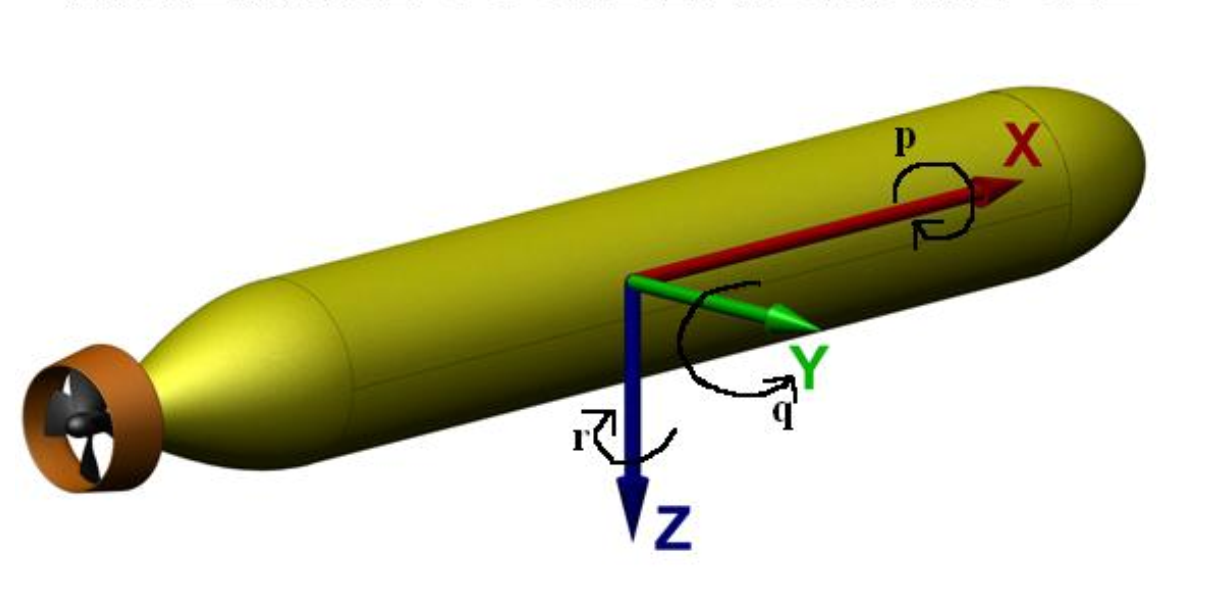
\includegraphics[width=0.4\linewidth]{figuras/revisaobiblio/coordenadasRPY}
	\label{fig:RPY}
	\fonte{Adaptado de \cite{diss:FabioAUV}.}
\end{figure}

Para aferir esses ângulos, em um sistema qualquer, é necessário o uso de sensores de posição inercial (IMU). Existem 3 modelos principais que são comumente usados de forma integrada para fornecer o máximo de precisão possível: Acelerômetro, Giroscópio e Magnetômetro. Todos esses serão obrigatórios para desenvolvimento do projeto proposto.

\subsubsection{Acelerômetro}

Acelerômetros são sensores que medem a aceleração de um sistema linearmente em relação a um eixo. Todas as forças envolvidas são mensuradas, como, por exemplo, a aceleração da gravidade \cite{diss:FabioAUV}, e o valor é dado em G ou $ (m/s^2) $. Por meio da força da gravidade, é possível decompor os vetores de força medindo a aceleração nos 3 eixos principais, e por meio disso calcular os ângulos inerciais de um objeto.

Um acelerômetro digital é um Sistema Micro Eletro Mecânico (MEMS) que funciona através da medição da capacitância entre duas aletas das estruturas internas, como demonstra a Figura \ref{fig:memnsacelerometer}. A alteração na capacitância corresponde à aceleração com que o bloco de massa interno se move \cite{site:MEMSHOTO}. 


\begin{figure}[!htb]
	\centering
	\caption{Visualização de um acelerômetro digital: a massa laranja se move, alternando a distância de sua aleta com as partes em verde, oscilando a capacitância C1 e C2}
	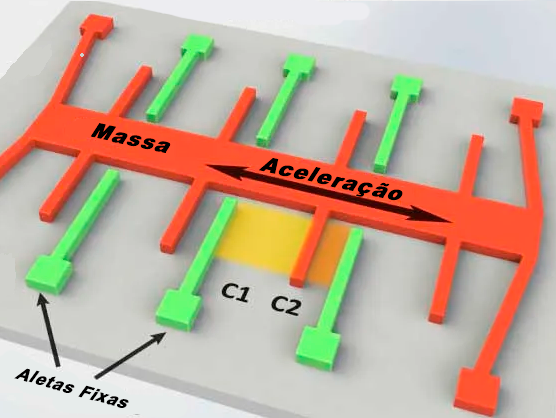
\includegraphics[width=0.7\linewidth]{figuras/revisaobiblio/memnsacelerometer}
	\label{fig:memnsacelerometer}
	\fonte{Adaptado de \cite{site:MEMSHOTO}.}
\end{figure}

\subsubsection{Giroscópio}

Giroscópios são sensores capazes de medir a taxa da variação angular de um corpo que gira em torno de um eixo e é mensurado em $ (^{\circ}/s) $ \cite{diss:FabioAUV}. Um giroscópio microeletrônico consiste em um ressonador, que vibra dentro de um espaço entre bases de apoio, detectando uma alteração na ressonância de acordo com o efeito de aceleração angular (Figura \ref{fig:memnsgyro}). Para obter o ângulo inercial de um objeto, considerando um giroscópio para cada eixo de rotação, é preciso integrar (somar) os valores de velocidade angular medidos ao longo do tempo \cite{tcc:viniciusPID2Graus}.


\begin{figure}[!htb]
	\centering
	\caption{Vista interna de um giroscópio digital}
	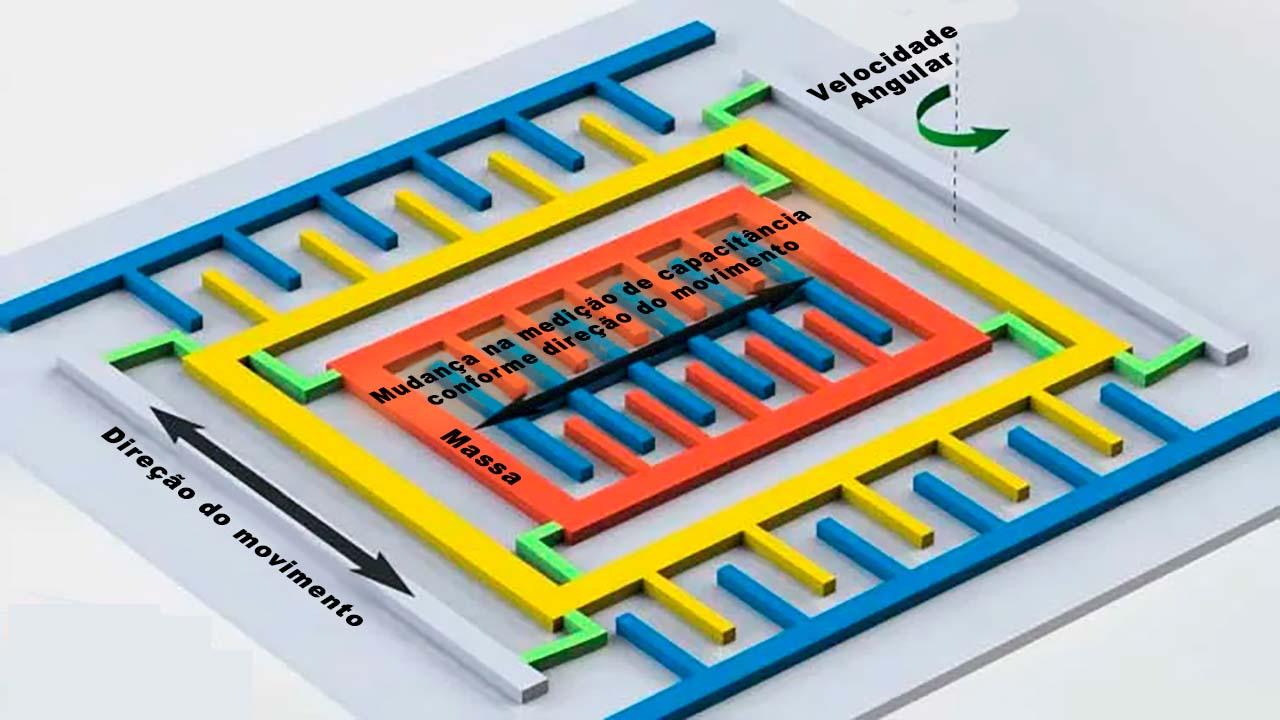
\includegraphics[width=0.7\linewidth]{figuras/revisaobiblio/memnsgyro}
	\label{fig:memnsgyro}
	\fonte{Adaptado de \cite{site:MEMSHOTO}.}
\end{figure}

\subsubsection{Magnetômetro}
Magnetômetros são sensores capazes de medir a intensidade do campo magnético em um eixo. Quando três magnetômetros são unidos para medir essa intensidade, um eixo cada, é possível determinar a direção e o sentido do campo magnético \cite{tcc:rafaelEESC}. Esses sensores são utilizados em pesquisas para verificar a intensidade do campo magnético terrestre, por exemplo. É por meio desse IMU que é possível construir uma bússola digital para realizar o alinhamento de um sistema para o polo Norte/Sul magnético do planeta.

Os magnetômetros digitais (MEMS) utilizam do Efeito Hall para medir a diferença de potencial gerada pelo caminho de passagem dos elétrons em um objeto metálico (Figura \ref{fig:memnsmag}). Alguns outros sensores usam do princípio da magneto-resistência, onde alguns metais (Ferro e Níquel) alteram sua resistência elétrica quando expostos a um campo magnético \cite{site:MEMSHOTO}.

%todo ver figura
\begin{figure}[!htb]
	\centering
	\caption{Efeito Hall aplicado para medição de campo magnético}
	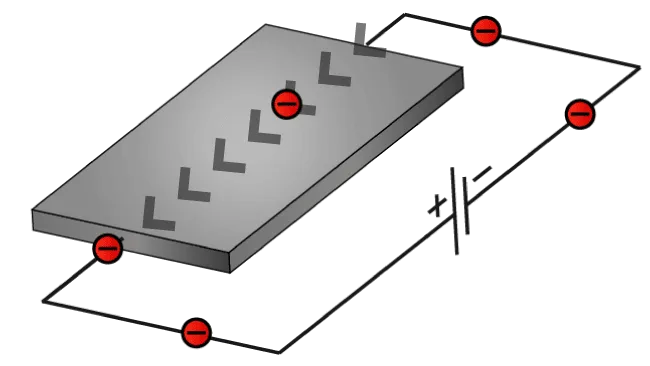
\includegraphics[width=0.7\linewidth]{figuras/revisaobiblio/memnsmag}
	\label{fig:memnsmag}
	\fonte{Adaptado de \cite{site:MEMSHOTO}.}
\end{figure}


\section{Processamento de Dados}

Infelizmente, os dados brutos fornecidos pelos sensores IMU, descritos nas seções anteriores, precisam passar por etapas de pós processamento, seja em \textit{hardware} ou \textit{software}, para que estejam livres de informações não desejadas, como ruídos. Além disso, é preciso transformar os dados de aceleração, velocidade e intensidade de campo magnético para determinar corretamente os ângulos de uma plataforma no sistema RPY. 

A partir do entendimento dos erros comuns em sensores IMU, é possível descrever boas práticas de análise e filtragem desses sinais. Uma abordagem secundária é realizar um pós processamento para combinar os valores de aceleração, velocidade angular e intensidade de campo magnético para que um sensor consiga compensar os erros dos demais, e obter um resultado mais preciso \cite{manual:cambimu}.

\subsection{Erros comuns em sensores IMU}

Sensores Inerciais não são totalmente exatos, independente do seu padrão de qualidade e podem carregar erros que comprometem um sistema de navegação. É preciso investigar a fonte dos erros, e compensar-los \cite{diss:FabioAUV}.

Erros gerados por imperfeições nos sensores são determinísticos e podem ser identificados e corrigidos na sua calibração. Mas além desses, existem outros distúrbios aleatórios que devem ser levados em conta no processo: \textit{Bias}, Ruído Branco e Efeitos de Temperatura.

\begin{itemize}
	\item \textbf{\textit{Bias}:} Sensores IMU possuem um erro de \textit{offset} que é chamado de \textit{bias}. Esse erro acompanha o valor bruto do sensor e pode gerar incongruências nas medições de ângulos. Em um giroscópio, quando a velocidade angular é integrada para calcular o ângulo de posição resultante, todos os erros ao longo do tempo acabam sendo somados e agregados no valor final \cite{manual:cambimu}. 
	
	\item \textbf{Ruído Branco:} esse tipo de erro é um ruído que acompanha o sinal de saída e pode ter origem no ambiente ou circuito do IMU. É um ruído que interfere em todo  espectro de frequência e pode ser minimizado utilizando filtros passa-baixa, passa-faixa ou passa-alta \cite{diss:FabioAUV}.
	
	\item \textbf{Efeitos de temperatura:} Todo acelerômetro e giroscópio é suscetível a uma não linearidade no efeito \textit{bias} devido a flutuações na temperatura. Contudo, é possível realizar calibrações para que o erro seja minimizado e isso requer um sensor de temperatura acoplado com o IMU \cite{manual:cambimu}. 
\end{itemize}

\subsection{Filtragem de sinais}

Um dos primeiros passos no processamento de dados é limpar o sinal cru do sensor, que agrega erros somando sinais que se originam em frequências de leitura indesejadas. Para isso, é preciso determinar qual a frequência de oscilação máxima do sistema e cortar qualquer dado que seja lido em uma frequência superior a de corte. Se esses valores não forem eliminados, os erros podem ser somados nas próximas etapas de pós processamento, acumulando e prejudicando o correto funcionamento do sistema \cite{article:Yang2017}.

A maneira mais comum de implementar isso é com um filtro passa-baixa, passa-faixa, ou passa-alta. Esses filtros são capazes de manter apenas o somatório de sinais dentro das frequências desejadas, rejeitando as demais em outras frequência. 

Filtro passa-baixa é o nome dado a um circuito eletrônico, ou algoritmo de processamento, que limita a amplitude dos sinais em frequências maiores que a frequência de corte, e mantém os demais inalterados. A quantidade de atenuação para cada frequência varia de acordo com as configurações adotadas no projeto do filtro, onde quanto maior a ordem do filtro, maior será a atenuação nas frequências fora da banda passante. 

Um filtro passa-altas, ao contrário, limita a amplitude dos sinais em frequências abaixo do corte. E o filtro passa-faixa é a combinação dos dois filtros anteriores, para permitir a passagem de sinais em frequências específicas.

Por meio desses filtros, portanto, é possível minimizar o impacto do ruído branco e eliminar possíveis distorções e vibrações que são indesejadas na leitura dos sensores \cite{article:Yang2017}. A frequência de corte e a ordem do filtro devem ser determinados pelo projetista de forma a garantir que os dados desejados não sejam afetados negativamente. 

\subsection{Cálculo de \textit{Pitch} e \textit{Roll}}

Uma vez que os sinais de acelerômetro e giroscópio tenham sido corretamente filtrados, é possível calcular os ângulos inerciais. Isso pode ser realizado de forma independente, usando os sensores de forma separada.

Uma vez que o acelerômetro esteja imóvel, e realizando a leitura somente da aceleração gravitacional, é possível calcular a posição inercial do sensor com os vetores de aceleração nos 3 eixos. Então, seja $ A_x $, $A_y$ e $A_z$ os dados relativos a cada eixo, as equações (\ref{apitch}) e (\ref{aroll}) correspondem, respectivamente a, o cálculo dos ângulos \textit{pitch} ($ \theta $) e \textit{roll} ($ \phi $) \cite{diss:coimbraSergio}. 

\begin{equation}
	\theta_A = \arctan\left(\dfrac{-A_x}{\sqrt{A_y^2+A_z^2}}\right) 
	\label{apitch}
\end{equation}

\begin{equation}
	\phi_A = \arctan\left(\dfrac{A_y}{A_z}\right)
	\label{aroll}
\end{equation}

O giroscópio, por outro lado, fornece os dados da taxa de variação angular dos 3 ângulos que se deseja obter. Dessa forma, a leitura dada pelo giroscópio é a derivada dos ângulos inerciais e, portanto, para calculá-los, basta realizar um somatório ao longo do tempo. Isso é descrito nas equações (\ref{gpitch}) e (\ref{groll}), considerando $G_{\theta}$ e $G_{\phi}$ os dados de cada eixo do giroscópio  \cite{diss:coimbraSergio}. 

\begin{equation}
	\theta_G = \int G_{\theta} dt
	\label{gpitch}
\end{equation}

\begin{equation}
	\phi_G = \int G_{\phi} dt
	\label{groll}
\end{equation}

\subsubsection{Filtro Complementar}

O Filtro Complementar é uma combinação linear na qual se define um peso para cada variável de entrada. Neste caso, um peso para o acelerômetro e outro para o giroscópio, em que a soma desses pesos deve ser igual a 1 \cite{tcc:viniciusPID2Graus}. 

A fusão de sensores é a solução para a combinação das faixas de precisão de ambos os sensores, a fim de um contornar a imprecisão do outro. O giroscópio é responsável pela medição precisa em comportamentos de alta frequência e o acelerômetro pela medição em baixas frequências \cite{artigo:forscienceKalman}. 

Então, é preciso definir a frequência de corte e os intervalos de medição dos sensores para calcular o valor da constante associada ao peso de cada sensor no cálculo final. Assim, para obter os ângulos de rotações, \textit{pitch} ($ \theta $) e \textit{roll} ($ \phi $), usa-se as equações (\ref{compfilterpitch}) e (\ref{compfilterroll}), sabendo que $ K_A + K_G = 1 $ \cite{tcc:viniciusPID2Graus}. 


\begin{equation}
	\theta =  K_A \cdot\theta_A + K_G\cdot\theta_G
	\label{compfilterpitch}
\end{equation}

\begin{equation}
	\phi =  K_A \cdot\phi_A + K_G\cdot\phi_G
	\label{compfilterroll}
\end{equation}

Onde, seja $ f_d $ a frequência de divisão desejada para os dados de acelerômetro e giroscópio e $ dt $ o intervalo entre as amostra de dados:

\begin{equation}
	K_G = \dfrac{\frac{1}{f_d}}{\frac{1}{f_d} + dt}
	\label{compfilterroll}
\end{equation}

\subsection{Magnetômetro como uma Bússola}

O campo magnético terrestre pode ser lido, em qualquer posição no planeta, como um vetor que aponta em direção ao polo norte magnético. Um magnetômetro pode ler os valores relativos aos seus 3 eixos e determinar o sentido do campo, como demonstrado na Figura \ref{fig:He}. A intensidade desse campo pode ser determinada pela equação (\ref{he}) \cite{man:Honeywell}.

\begin{figure}[!htb]
	\centering
	\caption{Vetor de direção do campo magnético}
	\includegraphics[width=0.3\linewidth]{figuras/revisaobiblio/He}
	\label{fig:He}
	\fonte{Adaptado de \cite{man:Honeywell}.}
\end{figure}

\begin{equation}
	H_e =  \sqrt{H_x^2 + H_y^2 + H_z^2}
	\label{he}
\end{equation}


Todo sistema de orientação com o campo magnético terrestre requer um sensor magnetômetro triaxial em conjunto com um sistema de medição inercial (Figura \ref{fig:magdiag}). O cálculo posicional da orientação magnética combina os dados dos 3 eixos de medição.

\begin{figure}[!htb]
	\centering
	\caption{Diagrama de leitura dos dados inerciais com magnetômetro}
	\includegraphics[width=0.7\linewidth]{figuras/revisaobiblio/diagrama}
	\label{fig:magdiag}
	\fonte{Adaptado de \cite{838300}.}
\end{figure}


Em uma situação de perfeitas condições, onde o sensor está alinhado com o plano horizontal e sem ruídos, é possível calcular o ângulo azimutal $ \psi $ pela equação (\ref{heading90g}), onde $ Y_h $ e $ X_h $ são os componentes horizontais da medição de campo magnético com o magnetômetro, como ilustra a figura \ref{fig:planihxhy}. O plano horizontal é definido pelo momento onde os dados de \textit{pitch} ($ \theta $) e \textit{roll} ($ \phi $) são nulos \cite{838300}.

\begin{equation}
	\psi = \arctan\left(\dfrac{Y_h}{X_h}\right)
	\label{heading90g}
\end{equation}

Em uma situação diferente, onde a plataforma se encontra inclinada (Figura \ref{fig:planihxhy}), é preciso decompor e planificar os vetores. Isso é feito com base nos dados de \textit{pitch} e \textit{roll} obtidos pelo acelerômetro e giroscópio. Após, reaplica-se os valores na equação (\ref{heading90g}) para determinar o azimute \cite{carusoSAE}. As equações (\ref{hx}) e (\ref{hy}) demonstram a planificação para cada componente horizontal, onde: $ Mx $, $ My $, $ Mz $ são os valores de campo magnético, para cada eixo, aferidos com o uso do magnetômetro.

\begin{figure}[!htb]
	\centering
	\caption{Planificação dos dados de um sistema inclinado}
	\includegraphics[width=0.7\linewidth]{figuras/revisaobiblio/xhyh}
	\label{fig:planihxhy}
	\fonte{Adaptado de \cite{838300}.}
\end{figure}

\begin{equation}
	X_h = M_x\cos(\theta) + M_y\sin(\phi)\sin(\theta) - M_z\cos(\theta)\sin(\phi)
	\label{hx}
\end{equation}

\begin{equation}
	Y_h = M_y\sin(\theta) + M_z\sin(\phi)
	\label{hy}
\end{equation}

\subsubsection{Distorções do campo magnético}

A precisão de sensores magnetômetros pode ser afetada pela presença de materiais ferrosos na proximidade, ou qualquer perturbação do campo magnético gerada por sistemas elétricos próximos. Para que o sensor consiga realizar uma leitura correta, é necessário calcular o quanto de perturbação está afetando a leitura do sensor.

Quando um componente ferroso é posicionado em um campo magnético uniforme, isso gera uma perturbação denominada \textit{hard-iron}. Porém, alguns materiais não magnéticos como ferro e níquel geram um erro chamado de \textit{soft-iron}. Ambos afetam o campo magnético de forma diferente, e precisam se compensados com estratégias de calibração, conforme à equação (\ref{eq:magerrorcalibration}), onde: $ Mn $ é uma matriz de erros de desalinhamento na montagem entre os eixos do sensor e do objeto; $S_x$, $S_y$, $S_z$ são fatores de escala; SI é a matriz composta de constantes para remover o erro \textit{soft-iron}; $R_x$, $R_y$, $R_z$ são os valores crus do sensor, e $O_x$, $O_y,$ $O_z$ são os \textit{offsets} causados pela interferência \textit{hard-iron} \cite{calibrationMatrix}.

\begin{equation}
	\left[\begin{array}{c}  M_x\\M_y\\M_z \end{array}\right] = \left[Mn\right]_{3x3} \cdot \left[\begin{array}{ccc} S_x&0&0\\ 0&S_y&0\\ 0&0&S_z \end{array}\right]\cdot \left[SI\right]_{3x3} \cdot \left[\begin{array}{c} R_x - O_x\\R_y - O_y\\R_z - O_z \end{array}\right]
	\label{eq:magerrorcalibration}
\end{equation}

Todas as constantes de calibração devem ser obtidas antes de fazer uso do sensor. Porém, os métodos para encontrar as constantes e aplicá-las pode divergir. Para este trabalho, concentrou-se em entender as calibrações no plano horizontal, pois, na prática, utilizar uma calibração nos 3 eixos poderia ser demasiado complexo não só para o controlador embarcado mas também implicaria em mais etapas e uma maior complexidade de usabilidade para o usuário final.


\subsubsection{Calibração contra erros \textit{hard} e \textit{soft-iron}}

Quando um conjunto de medições é feita rotacionando um magnetômetro $ 360^{\circ} $, é possível obter um mapa planificado do campo magnético ao redor do sensor. Na Figura \ref{fig:magnormal} é visível um campo sem interferências, formando um círculo com os dados coletados. Quando uma interferência \textit{hard-iron} ocorre, o campo magnético é alterado com um \textit{offset} (Figura \ref{fig:hardiron}) que é simples de ser detectado por um controlador. Diferentemente, a interferência \textit{soft-iron} manipula o campo e distorce o círculo, formando uma elipse (Figura \ref{fig:softiron}). Quando ambas as distorções são combinadas, o campo é lido como uma elipse fora de centro \cite{site:magFierce}. 


\begin{figure}[!htb]
	\centering
	\caption{Leitura de dados ideal de um magnetômetro ao rotacioná-lo  $ 360^{\circ} $}
	\includegraphics[width=\linewidth]{figuras/revisaobiblio/magnormal}
	\label{fig:magnormal}
	\fonte{Adaptado de \cite{man:HSIcalibration}.}
\end{figure}

\begin{figure}[!htb]
	\centering
	\captionsetup[subfigure]{justification=centering}
	\caption{Impacto das interferências \textit{hard-iron} (a) e  \textit{soft-iron} (b) na leitura do magnetômetro em rotação de $ 360^{\circ} $}
	\begin{subfigure}[b]{0.49\textwidth}
		\centering
		\includegraphics[width=.9\linewidth]{figuras/revisaobiblio/hardiron}
		\caption{}
		\label{fig:hardiron}
	\end{subfigure}
	\hfill
	\begin{subfigure}[b]{0.49\textwidth}
		\centering
		\includegraphics[width=.9\linewidth]{figuras/revisaobiblio/softiron}
		\caption{}
		\label{fig:softiron}
	\end{subfigure}
	\label{}
	\fonte{Adaptado de \cite{man:HSIcalibration}.}
\end{figure}


O método mais simples de ser implementado é compensando somente a distorção \textit{hard-iron}. Para isso, é preciso determinar os \textit{offset} da distorção $O_x$, $O_y$, $O_z$ medindo a distância da extremidade ao centro do círculo, para cada eixo. Isso é demonstrado respectivamente nas equações (\ref{ox}) e (\ref{oy}), onde os valores mínimos e máximos são os menores e os maiores valores obtidos da leitura crua do magnetômetro, enquanto é rotacionado $ 360^{\circ} $ \cite{site:magFierce}.  

\begin{equation}
	O_x = \dfrac{x_{max} + x_{min}}{2}
	\label{ox}
\end{equation}

\begin{equation}
	O_y = \dfrac{y_{max} + y_{min}}{2}
	\label{oy}
\end{equation}

Porém, esse algoritmo não elimina a distorção \textit{soft-iron}. Para isso, pode-se usar os mesmos valores mínimos e máximos mencionados anteriormente. E, a partir deles, trabalhando somente no plano horizontal, é possível determinar os fatores de escala $ S_x $ e $ S_y $, além dos \textit{offsets} $ O_x $ e $ O_y $, como demonstram as equações (\ref{xsf}), (\ref{ysf}), (\ref{xoff}) e (\ref{yoff}). Os fatores de escalas, se calculados menores que 1, devem ser aproximados para 1 \cite{carusoSAE}.

\begin{equation}
	S_x = \dfrac{(y_{max} - y_{min})}{(x_{max} - x_{min})}
	\label{xsf}
\end{equation}

\begin{equation}
	S_y = \dfrac{(x_{max} - x_{min})}{(y_{max} - y_{min})}
	\label{ysf}
\end{equation}

\begin{equation}
	O_x = \left[\dfrac{(x_{max} - y_{min})}{2} - x_{max} \right] \cdot S_x
	\label{xoff}
\end{equation}

\begin{equation}
	O_y = \left[\dfrac{(y_{max} - y_{min})}{2} - y_{max} \right] \cdot S_y
	\label{yoff}
\end{equation}

Dessa maneira, apenas com foco no plano horizontal, e desconsiderando erros de desalinhamento na montagem, a equação (\ref{eq:magerrorcalibration}) é simplificada em (\ref{eq:magerrorcalibrationfinal2}) e (\ref{eq:magerrorcalibrationfinal2}); a matriz de compensação do erro \textit{soft-iron} é substituída somente pelos fatores de escala. E, assim, o azimute pode ser determinado pela equação (\ref{heading90gfinal}) .

\begin{equation}
	\left[\begin{array}{c}  M_x\\M_y \end{array}\right] = \left[\begin{array}{cc} S_x&0\\ 0&S_y \end{array}\right] \cdot \left[\begin{array}{c} R_x - O_x\\R_y - O_y\end{array}\right]
	\label{eq:magerrorcalibrationfinal1}
\end{equation}

\begin{equation}
	\left[\begin{array}{c}  M_x\\M_y \end{array}\right] = \left[\begin{array}{c} S_x \cdot\left(R_x - O_x\right)\\ S_y \cdot\left( R_y - O_y\right)\end{array}\right]
	\label{eq:magerrorcalibrationfinal2}
\end{equation}

\begin{equation}
	\psi = \arctan\left(\dfrac{M_y}{M_x}\right)
	\label{heading90gfinal}
\end{equation}

Esse algoritmo já foi aplicado por \cite{carusoSAE} no processo de calibração de magnetômetros dentro de veículos, para remover a distorção provocada pelos materiais do carro e do motor. A Figura \ref{fig:caruso} demonstra a efetividade desse procedimento.

\begin{figure}[!htb]
	\centering
	\captionsetup[subfigure]{justification=centering}
	\caption{Aplicação da calibração: (a) sinal original lido, (b) sinal lido após aplicação da calibração}
	\begin{subfigure}[b]{0.49\textwidth}
		\centering
		\includegraphics[width=.9\linewidth]{figuras/revisaobiblio/carusodistorcion}
		\caption{}
		\label{fig:carusodistorcion}
	\end{subfigure}
	\hfill
	\begin{subfigure}[b]{0.49\textwidth}
		\centering
		\includegraphics[width=.9\linewidth]{figuras/revisaobiblio/carusoclean}
		\caption{}
		\label{fig:carusoclean}
	\end{subfigure}
	\label{fig:caruso}
	\fonte{Adaptado de \cite{carusoSAE}.}
\end{figure}

Por fim, é crucial cuidar a instalação do sensor, que deve estar o mais afastado possível de motores, materiais magnéticos e ferrosos | principalmente ferro e níquel |. Se isso não for possível, que seja determinada a distorção gerada pelos componentes para realizar o \textit{offset}. Porém, mesmo com calibração, não é possível eliminar a distorção de medições em função de campos magnéticos oscilantes \cite{838300}. 

E, além disso, ressalta-se que as distorções magnéticas ocorrem conforme o sistema é posicionado em locais diferentes, e cada local deve ter sua própria calibração. Se o sensor é reinstalado em outra orientação no mesmo local, então também será necessário uma nova calibração. Somente após todas essas etapas é possível identificar o correto sentido do norte magnético terrestre \cite{838300}. 

\section{Protocolos de Comunicação Serial}

O sensores e atuadores explicados nas seções anteriores podem se comunicar com os controladores através de protocolos de comunicação específicos. Esses modelos funcionam como uma linguagem para acessar as informações, sendo fundamentais para a diagramação do sistema eletrônico em \textit{hardware} e \textit{software}. Por meio dessas redes, um controlador consegue realizar a leitura dos dados armazenados no registrador de um sensor, por exemplo, ou escrever uma nova calibração em outro local da memória \cite{man:texasI2C}.

\subsection{UART}
O protocolo UART (\textit{Universal Asynchrounous Receiver/Transmiter}) é uma forma de comunicação baseada em padrões industriais. Nesse protocolo há somente duas linhas: receptor (RX) e transmissor (TX) que utilizam de uma taxa de transmissão referência (\textit{baud rate}) para que haja o correto processamento bit a bit do que é comunicado via protocolo \cite{man:texasUART}. 

As mensagens enviadas possuem limite na velocidade que depende do \textit{clock} do controlador que está sendo utilizado. Além disso, baseado nas configurações dos dispositivos, as mensagens são enviadas no seguinte pacote (Figura \ref{fig:uartcommunication}):

\begin{itemize}
	\item 1 \textit{START bit}
	\item 5, 6, 7, ou  8 \textit{data bits}
	\item 1 \textit{PARITY bit} (opcional)
	\item 1, 1.5, ou \textit{2 STOP bits}
\end{itemize}

\begin{figure}[!htb]
	\centering
	\caption{Exemplos de comunicação UART}
	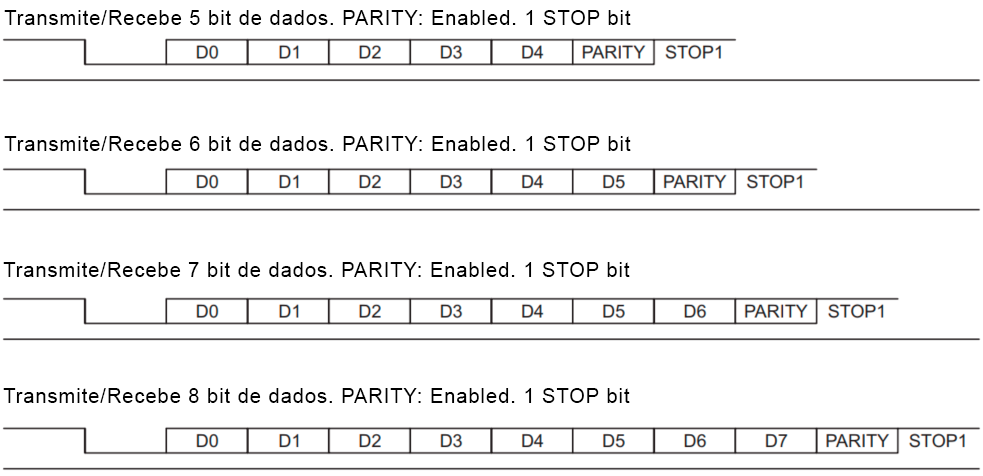
\includegraphics[width=\linewidth]{figuras/revisaobiblio/uartcommunication}
	\label{fig:uartcommunication}
	\fonte{Adaptado de \cite{man:texasUART}.}
\end{figure}

Os pinos de comunicação UART são conectados ligando-se o pino RX de um dispositivo no TX do outro. O projeto do \textit{hardware} dessas linhas de comunicação é um pouco mais livre, mas recomenda-se manter a indutância tão baixa quanto possível, além de rotear as trilhas de comunicação afastadas das fontes de ruído \cite{site:altiumpcb}.

\subsection{I2C}

A rede I2C (\textit{Inter-Integrated Circuit}) é um protocolo padrão e popular, usado para comunicação entre mestre(s) e escravo(s) (Figura \ref{fig:i2connection}). 
Para a comunicação ocorrer, o mestre deve ordenar quando e o que será transmitido pelos escravos. Nesse procedimento, o mestre sempre especifica o endereço do escravo que ele deseja ler ou escrever alguma informação nos seus registradores, esses endereços são um valor de 0 a 127 e dois escravos não devem partilhar o mesmo valor \cite{man:texasI2C}. A rede permite diversos modos de comunicação, que se diferenciam pela velocidade da transmissão de dados. Os mais comuns são de 100 kbit/s (\textit{Standard Mode}), 400 kbit/s (\textit{Fast Mode}) ou 3.4 Mbit/s(\textit{Fast Mode Plus}). Contudo, nem todos os dispositivos que aceitam o protocolo I2C irão suportar todos os modos obrigatoriamente.

\begin{figure}[!htb]
	\centering
	\caption{Topologia de uma rede I2C com 1 mestre e 3 escravos conectados às linhas SDA e SCL, ambas com resistores de \textit{pull-up}}
	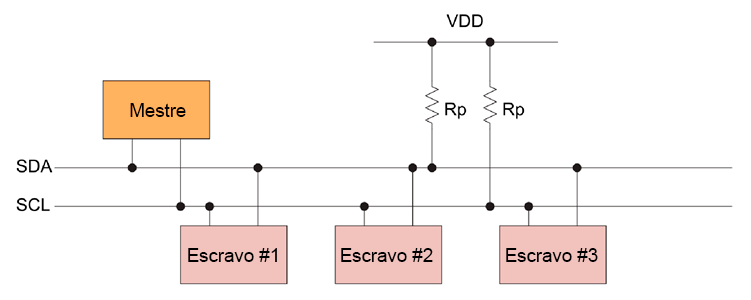
\includegraphics[width=0.7\linewidth]{figuras/revisaobiblio/i2connection}
	\label{fig:i2connection}
	\fonte{Adaptado de \cite{site:analogI2c}.}
\end{figure}

Para funcionar, o protocolo I2C precisa de duas linhas: \textit{Serial Data} (SDA) e \textit{Serial Clock} (SCK ou SCL) (Figura \ref{fig:i2connection}). Essas linhas precisam estar conectadas com a alimentação do sistema, que deve ser de 5V, por meio de um resistor \textit{pull-up}. O valor mínimo dele é calculável com a equação (\ref{pullupi2cmin}), considerando $ V_{OL} $ e $ I_{OL} $ a tensão e corrente máxima para que os circuitos consigam realizar a leitura de um nível lógico válido \cite{man:texasI2Cpullup}. 

\begin{equation}
	R_P(min) = \dfrac{ V_{CC} - V_{OL}(max) }{I_{OL}}
	\label{pullupi2cmin}
\end{equation}

Contudo, existe um valor limite para o resistor, que é determinado pelo total da capacitância entre as linhas. Esse fator altera o tempo de alternância entre um nível lógico alto e baixo, que deve estar dentro de padrões da rede. Esse tempo máximo depende da taxa de transmissão, ou modo da rede. Assim, $ t_r=1000ns  $ (\textit{Standard Mode}), $ t_r=300ns $ (\textit{Fast Mode}) e $ t_r=120ns  $ (\textit{Fast Mode Plus}). Esse valor máximo é determinado pela equação (\ref{pullupi2cmax}) \cite{man:texasI2Cpullup}.

\begin{equation}
	R_P(max) = \dfrac{ t_r }{0,8473 \times C_b}
	\label{pullupi2cmax}
\end{equation}

A transmissão de dados se inicia quando a rede está em \textit{idle}, ou seja, ambas as linhas devem estar em nível lógico alto após uma condição de STOP (nível lógico baixo). Dessa maneira, considerando dois cenários possíveis, a comunicação pode ser prosseguida das seguintes formas: o mestre deseja escrever ou alterar dados no escravo; o mestre deseja ler dados de um escravo \cite{man:texasI2C}.

\begin{enumerate}
\item Para o primeiro caso (Figura \ref{fig:i2cwrite}):
\begin{itemize}
	\item Mestre transmite uma condição de \textit{START} e envia o endereço do escravo com quem quer se comunicar;
	\item Mestre envia os dados;
	\item A transferência se encerra com um sinal de \textit{STOP} do mestre.
\end{itemize}

\item Para o segundo caso  (Figura \ref{fig:i2cread}):
\begin{itemize}
	\item Mestre transmite uma condição de \textit{START} e envia o endereço do escravo com quem quer se comunicar;
	\item Mestre solicita uma leitura de dados no registrador do escravo;
	\item Escravo envia os dados para o Mestre;
	\item Mestre encerra a transmissão com sinal de \textit{STOP}.
\end{itemize}
\end{enumerate}

\begin{figure}[!htb]
	\centering
	\caption{Transmissão de dados do mestre para o escravo}
	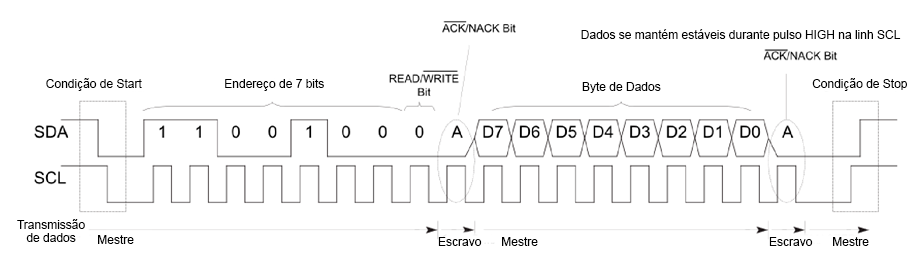
\includegraphics[width=1\linewidth]{figuras/revisaobiblio/i2cwrite}
	\label{fig:i2cwrite}
	\fonte{Adaptado de \cite{site:analogI2c}.}
\end{figure}

\begin{figure}[!htb]
	\centering
	\caption{Requisição de dados do mestre ao escravo}
	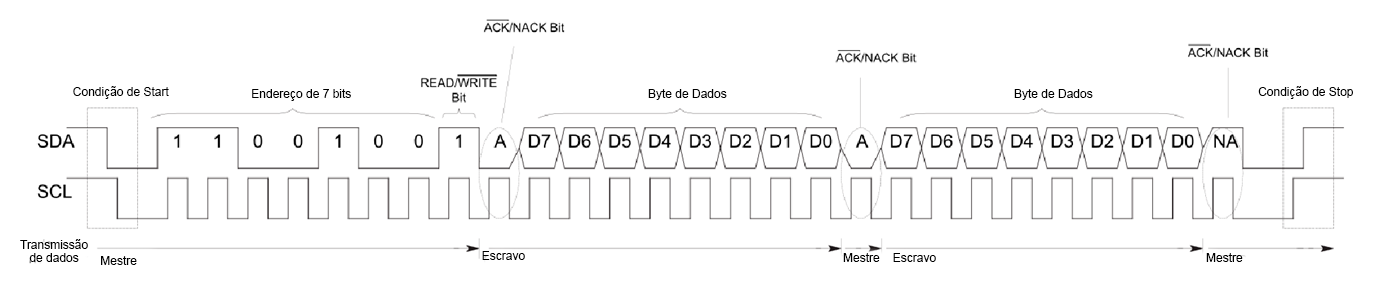
\includegraphics[width=1\linewidth]{figuras/revisaobiblio/i2cread}
	\label{fig:i2cread}
	\fonte{Adaptado de \cite{site:analogI2c}.}
\end{figure}


As condições de \textit{START} e \textit{STOP} são descritas sempre pelo mestre. Essas duas condições são situações específicas na rede, pois são o único momento da transmissão em que a linha SDA é alterada enquanto o \textit{clock} na linha SCK está em nível lógico alto. No caso de uma situação de \textit{START}, a linha SDA alterna do nível lógico alto para o baixo, e o inverso ocorre na situação de \textit{STOP} (Figura \ref{fig:startstopconditioni2c}) \cite{site:analogI2c}.

\begin{figure}[!htb]
	\centering
	\caption{condições de \textit{START} e \textit{STOP} no padrão I2C}
	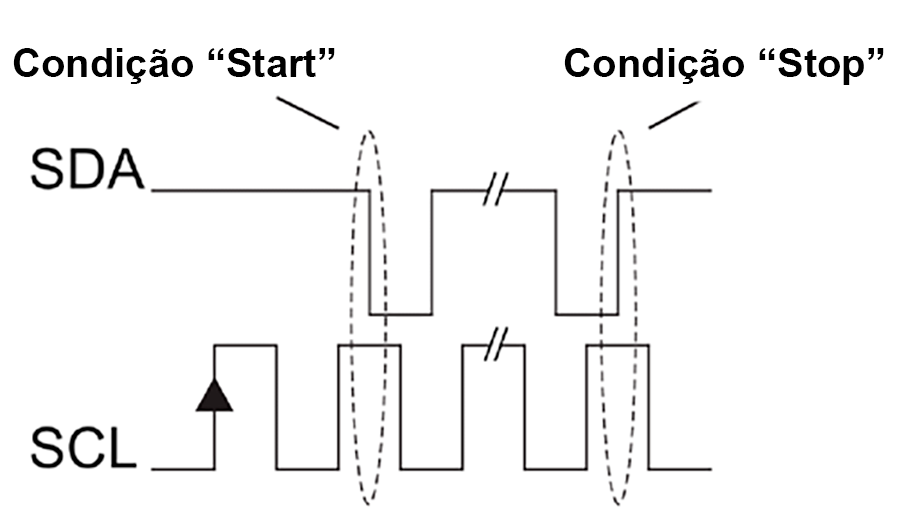
\includegraphics[width=0.65\linewidth]{figuras/revisaobiblio/startstopconditioni2c}
	\label{fig:startstopconditioni2c}
	\fonte{Adaptado de \cite{site:analogI2c}.}
\end{figure}

Para cada conjunto de dados enviados, um bit ACK (\textit{acknowledgement}) é enviado na sequência - lido como um nível lógico baixo - pelo receptor da mensagem, comunicando o correto recebimento e permitindo uma nova transmissão. Esse bit é enviado imediatamente após a comunicação, e o transmissor deve liberar a linha SDA para que o receptor possa enviar a mensagem \cite{man:texasI2C}. 

Devido ao controle de impedância e capacitância, recomenda-se que o roteamento físico desses sinais, em uma placa de circuito, não seja longo. Quanto maior a velocidade de comunicação, menor deve ser a distância entre os dispositivos I2C, afastando-os também de sistemas que possam causar interferência eletromagnética \cite{site:altiumpcb}.

\subsection{Bluetooth}

\textit{Bluetooth} é um protocolo de comunicação sem-fio e de curto alcance. Esse sistema é uma tecnologia adequada para sistemas embarcados por apresentar um baixo custo e consumo, provendo fácil conectividade, sobretudo nas versões mais recentes do protocolo \cite{diss:ClaudioBluetooth}. 

O fator baixo consumo aumenta a economia de energia e limita o alcance da conexão a depender da classe do dispositivo. Para um dispositivo Classe 3, com 1mW de potência, o alcance será de até 1 m; classe 2, com até 10 mw, alcance de 1 0m; classe 3, com até 100 mW, total de 100 m \cite{tcc:tier2019}.

A tecnologia \textit{wireless} \textit{bluetooth} especifica um modelo de comunicação síncrono entre somente um par de dispositivos com a banda de 2.4 GHz a 2.5 GHz dividida igualmente entre eles. Esse padrão já é geralmente usado para sistemas de localização, transferência de áudio e dados de forma geral \cite{book:BluetoothDemystified}.

Nesse protocolo, cada dispositivo possui um endereço MAC (\textit{Media Access Control} ou Controle de Acesso de Mídia) que distingue-os, sendo gravado fisicamente no \textit{hardware}. Aquele que solicita a comunicação passa a ser o mestre de uma relação mestre/escravo, que também é \textit{full-duplex} \cite{diss:ClaudioBluetooth}. 

Quando dois ou mais dispositivos se conectam via \textit{Bluetooth}, um deles será o mestre e será formada uma \textit{Bluetooth Wireless Personal Area Network} (BT-WPAN). Será classificada como \textit{piconet} para até 8 dispositivos conectados e \textit{scatternet} caso duas redes \textit{piconet} se comuniquem por meio de um dispositivo escravo de cada uma \cite{tcc:tier2019}. 

\subsubsection{Bluetooth Low Energy}

\textit{Bluetooth Low Energy} (BLE) é uma versão da tecnologia otimizada para baixo consumo e é atualmente muito utilizado em \textit{smartphones}. Para que a tecnologia funcione, otimizando a comunicação, é definido um protocolo para diferentes perfis com atributos genéricos de dispositivos (GATT do inglês \textit{Generic Attribute Profile}). Os perfis GATT correspondem a serviços e características \cite{man:btlecore52}.

Os serviços servem para caracterizar os conjuntos de dados, por exemplo um sensor de batimento cardíaco. A característica do perfil define uma propriedade ou configuração da informação. Em uma analogia, o GATT é como entrar em uma sala de armazenamento com vários armários e cada armário com várias gavetas. Nesse caso, os serviços são os armários e as gavetas são as características com as informações dos dispositivos \cite{site:devzonebtle}.

Na comunicação, todas essas informações são identificadas por um código único, ou \textit{Universally Unique ID} (UUID). Esse é um valor que identifica o tipo de dispositivo com o qual um \textit{smartphone}, por exemplo, está se comunicando, e descreve todas as informações mencionadas anteriormente. Existem padrões UUID de 16 bits como para o caso do sensor de batimento cardíaco. Mas para dispositivos que não seguem um padrão, existem UUIDs de 128 bits que servem para caracterizar serviços específicos em aplicações únicas \cite{site:devzonebtle}. Por meio desses UUIDs que um dispositivo consegue reconhecer qual o tipo de dado que está sendo comunicado, e assim o protocolo pode se otimizar para melhor atender à demanda da comunicação.

\section{Interface Gráfica}
Para que um sistema embarcado se torne amigável para um usuário comum, é preciso uma interface gráfica que sintetize as informações e forneça formas de controle do usuário para a plataforma. Exemplos de interfaces podem ser simples botões, LEDs ou também um aplicativo para \textit{smartphone}. Contudo, independente do nível de complexidade, toda interface deve se ater a princípios em sua elaboração, para que se tornem entendíveis pelo maior número possível de usuários.

\subsection{Princípios e Diretrizes}

Os princípios e as diretrizes comumente utilizados em interfaces humano-computador giram em torno dos seguintes tópicos: correspondência com as expectativas dos usuários; simplicidade nas estruturas das tarefas; equilíbrio entre controle e liberdade do usuário; consistência e padronização; promoção da eficiência do usuário; antecipação das necessidades do usuário; visibilidade e reconhecimento; conteúdo relevante e expressão adequada; e projeto para erros \cite{BarbosaEtAl2021InteracaoHumanoComputadorExperiencia}.
Esse conjunto de princípios são conhecidos como heurística de Nielsen, pois são aplicáveis em qualquer sistema, independente de casos específicos.

\subsubsection{Visibilidade dos status do sistema}

O sistema deve sempre manter o usuário atualizado sobre as condições de operação com uma taxa de atualização condizente para a informação. Ao informar o status da bateria, por exemplo, o usuário do \textit{smartphone} consegue predizer quanto tempo de uso ainda terá e irá conseguir manejar sua interação com base nessa previsibilidade \cite{site:nielsen}.

\subsubsection{Comunicar-se com o mundo real}
O Projeto tem que se comunicar com o usuário na língua do usuário. Se um brasileiro não sabe inglês, ele "ficará perdido" nos Estados Unidos. Da mesma forma, o desenvolvedor não pode assumir que o usuário entenderá o aplicativo somente pelo fato do desenvolvedor ter feito algo que ele próprio entenda. É sempre recomendado conferir a linguagem do sistema com um conjunto grande de pessoas para evitar mal entendidos.

Quando o usuário não entende a língua do sistema, ele se sente afastado e irá deixar de usar a plataforma. É interessante que a plataforma tenha \textit{designs} semelhantes com objetos do mundo real, dessa forma, o usuário se sente "contemplado" e consegue facilmente fazer a conexão entre o mundo real e a plataforma \cite{site:nielsenRealWorld}.

\subsubsection{Liberdade de Controle do Usuário}

Por vezes, a pessoa que está realizando um processo em um sistema pode cometer um engano. Esse evento pode levar a situações de erro que não devem comprometer a experiência. Por isso, os usuários precisam de uma “saída de emergência” claramente marcada para sair do estado indesejado. Isso reduz a sua ansiedade e o medo de errar, pois ele sabe que os erros podem ser contornados \cite{BarbosaEtAl2021InteracaoHumanoComputadorExperiencia}.

\subsubsection{Consistências e Padrões}

É importante que o sistema mantenha uma consistência entre suas telas, ou mesmo em grandes plataformas, ou seja, que os múltiplos programas tenham o mesmo padrão, com funções localizadas no mesmo lugar, com nomes similares e com um \textit{disign} similar. Exemplo disso são as telas dos aplicativos do Google Docs: todos possuem o mesmo estilo de menu. Idem para o Microsoft Office.

A consistência também se estende aos ícones. O ícone que representa um botão, por exemplo, é importante que seja consistente em estilo com os demais. Eles podem ser mais preenchidos, \textit{clean}, neutros ou suaves. O que importa nesse caso, é que sejam todos padronizados \cite{site:nielsenIcon}.


\subsubsection{Prevenção de erros}

Uma forma de prevenção é oferecer sugestões numa caixa de pesquisa, por exemplo. Em situações de rotina, como disparar um lembrete, a tela de criação pode oferecer uma sugestão padrão de um modelo que faça sentido para o usuário. Para evitar corrupção de dados pelo usuário durante o cadastro, é possível sugerir ao usuário o preenchimento de números de forma truncada, fazendo o pós-processamento para ler o número corretamente.

\subsubsection{Relembrar o usuário é mais fácil do que o usuário relembrar}

Quando o usuário precisa repensar sobre algo incomum na memória, ele despende muito tempo. Então, quando a plataforma exige uma lembrança do usuário para entender algo, isso limita a experiência e incorre em perda de tempo ou confusão.

Por isso, é mais interessante realizar a exigência com uma possível sugestão de resposta correta. A recognição de algo é muito mais prático para a mente humana, pois ao mostrar para o cérebro algo relacionado com o que precisa lembrar-se, dispara-se a memória de forma mais efetiva. Dar uma pista para o cérebro é mais eficiente do que simplesmente perguntar sem oferecer nada \cite{site:nielsenRecall}.

\subsubsection{Torne o sistema flexível e eficiente}

Atalhos, personalização e customização. Com esses fatores é possível melhorar a usabilidade para aqueles que não são mais novatos no \textit{software} e isso ajuda a manter esses usuários ativos. Um fotógrafo experiente, que está acostumado com os atalhos de teclado nos aplicativos da Adobe, teria muita dificuldade se o teclado viesse a falhar, pois a mente já assimilou os atalhos mais usados e eles fazem diferença na velocidade com que o profissional interage com o \textit{software} \cite{site:nielsenFlexibility}.

\subsubsection{Tenha um projeto minimalista}

Um projeto é minimalista significa usar elementos simples num arranjo onde desenho e a interface combinem de forma agradável sem chamar a atenção de forma desnecessária, colaborando com que o usuário foque somente naquilo que é necessário \cite{site:nielsen}.

\subsubsection{Ajude o usuário a entender e se recuperar de erros}

O usuário precisa entender quando o sistema não está funcionando bem e como fazê-lo voltar à normalidade. As mensagens de erro devem ser expressas de uma forma simples, indicando o possível problema e a solução. 
Cores vermelhas e pretas ajudam a demonstrar o sinal de erro para o usuário \cite{site:nielsenError}.

\subsubsection{Tire dúvidas e documente o sistema}

Existem duas formas de ajudar o usuário e tirar suas dúvidas. A primeira é de forma proativa, onde a aplicação guia o usuário para se familiarizar com a interface. Outra forma é por uma seção com perguntas e respostas, a qual ajuda os usuários a se tornarem mais independentes com a aplicação, resolvendo seus próprios problemas e filtrando os casos que precisam de suporte para a equipe técnica da plataforma \cite{site:nielsenHelpandDoc}.

\subsection{Android}
Para desenvolver o aplicativo de controle que o usuário final irá utilizar no processo de alinhamento da plataforma, será usado o \textit{framework} \textit{Android}, da \textit{Google}.

\subsubsection{Ambiente de Desenvolvimento}

O \textit{Android Studio} é o ambiente de desenvolvimento integrado oficial para a criação de aplicativos \textit{Android} e é baseado no \textit{IntelliJ IDEA}. Ele oferece uma série de Recursos que possibilitam a confecção de um aplicativo: Sistema de compilação flexível baseado em \textit{Gradle}; Um emulador rápido com suporte a vários recursos; ambiente unificado que possibilita o desenvolvimento para qualquer dispositivo \textit{Android}, incluindo relógios e televisões; integração com \textit{GitHub} para \textit{backup} e documentação do código; entre outras funções que possibilitam analisar o desempenho de um aplicativo em tempo real, bem como fazer \textit{updates} \cite{site:androidstudio}.

\subsubsection{Linguagens de Programação}

Existem soluções de desenvolvimento \textit{Android} mais \textit{user-friendly} como \textit{APP Inventor} ou \textit{Kodular}, porém, essas interfaces não garantem ao desenvolvedor um pleno controle do aplicativo, e muitas vezes acabam limitando o projeto da interface. Por isso, usar linguagens de programação nativas é uma abordagem mais interessante para aplicativos mais completos. É possível criar aplicativos com diversas linguagens, mas somente duas são nativas e permitem realizar aplicações que podem usar de todo o poder de processamento de um \textit{smartphone}: Java e \textit{Kotlin}.

Em 2017, \textit{Kotlin} foi definido pela Google como sendo a principal linguagem de desenvolvimento \textit{Android}. Ela é muito mais nova que Java, sendo desenvolvida pela JetBrains. A grande motivação de se usar \textit{Kotlin} para o desenvolvimento reside no fato de ser uma linguagem segura para prevenção de objetos nulos, operando em paralelo com qualquer código em Java e dando opções de co-rotinas. Além disso, ao comparar dois códigos com a mesma função, um escrito em Java e o outro em \textit{Kotlin}, o segundo pode ser até 40\% mais compacto, o que implica em uma linguagem mais concisa e compreensível entre desenvolvedores. A desvantagem de se usar \textit{Kotlin}, para este trabalho, é somente a falta de uma comunidade grande, comparando com Java, o que limita o suporte para eventuais problemas de desenvolvimento \cite{site:kotlinxjava}.

Dentro do ambiente de desenvolvimento usa-se também linguagem de arquivos XML para a criação de interfaces gráficas (\textit{layouts}), bem como a escrita dos vetores, animações, e arquivos de configuração do aplicativo e temas de \textit{layout}. Para armazenamento de dados dentro do aplicativo, normalmente usa-se um banco de dados que é operado com códigos de consulta \textit{SQL}.

\subsubsection{\textit{Material Design}}
Existem uma série de diretrizes de projeto fornecidas pela Google para guiar o desenvolvimento de aplicativos \textit{Android}. Essas informações são fornecidas principalmente pela biblioteca \textit{Material Design}, que fornece pacotes facilmente implementáveis de \textit{layouts} para aplicações responsivas e padronizadas.

A biblioteca colabora com o desenvolvedor fornecendo ícones, tipografia, cores e componentes gráficos que trazem uma imersão para o usuário de forma simples e minimalista. Os \textit{designs} se inspiram no mundo real, facilitando a comunicação com o usuário \cite{site:materialdesign}.

\subsection{Usuários}

O objetivo deste trabalho possui um nicho muito específico de usuários: astrofotógrafos. Dentro desse grupo de pessoas, é possível abstrair uma série de expectativas e necessidades a respeito desse sistema e, mais especificadamente, de uma interface. Para entender o ponto de vista dos possíveis usuários é preciso criar pesquisas buscando uma coleta de dados relevantes para o projeto. 

No entanto, é importante destacar que o termo "usuário" não diz respeito somente a um astrofotógrafo que realmente irá usar a plataforma. Ele pode ser não só um usuário ativo (primário), ou um ocasional (secundário), mas também pessoas entusiastas que acompanham a astrofotografia e são chamados de \textit{stakeholders} \cite{BarbosaEtAl2021InteracaoHumanoComputadorExperiencia}.

A partir da análise feita com a coleta de dados inicial, é possível determinar as exigências de \textit{software} (e também \textit{hardware}) que implicam na melhor usabilidade da plataforma equatorial. E ressalta-se a importante dos testes, não somente em código, mas também com múltiplos usuários, fazendo uma análise de possíveis problemas de interface.